% Лабораторная работа по информатике № 1
% Михедов Константин Константинович БИБ224

%Тип документа: статья, размер бумаги - A4, написано 14 кегелем
\documentclass[a4paper]{article}

% Поиск по скомпилированному PDF
\usepackage{cmap}
% Кодировка выходного текста
\usepackage[T2A]{fontenc}
% Кодировка исходного текста
\usepackage[utf8]{inputenc}
% Поддержка необходимых языков
\usepackage[english,russian]{babel}

% Поддержка изображений
\usepackage{graphicx}
% Путь до внешних изображений
\graphicspath{ {./figures/}}

% Умная запятая
\usepackage{icomma}

% Ссылки на электронные ресурсы
\usepackage{hyperref}
% Настройка внешнего вида ссылок
\hypersetup{
  % Отключить прямоугольную рамку
  pdfborder={0 0 0},
  % Включить цветные ссылки
  colorlinks=true,
  % Цвет для ссылок на веб-ресурсы
  urlcolor=blue,
  % Цвет внутренних ссылок
  linkcolor=black
}

% Дополнительная математика
\usepackage{amsmath,amsfonts,amssymb,amsthm,mathtools}
% Показывать номера только у тех выржений, на которые кто-то ссылается
\mathtoolsset{showonlyrefs=true}

% Дополнительные символы
\usepackage{mathbbol}

% Правильное оформление
% Настройка отступов
\usepackage[left=2cm,right=1cm,top=2cm,bottom=2cm]{geometry}
% Настройка шрифта
\usepackage{fontspec}
\usepackage[fontsize=14pt]{fontsize}
\setmainfont{Times New Roman}
% Настройка межстрочных интервалов
\usepackage{setspace}
\onehalfspacing
% и межабзацных
\usepackage{parskip}
\setlength{\parindent}{1.25cm} 

% Красная строка
\usepackage{indentfirst}
\setlength{\parindent}{1.25cm} 

% Корректное положение рисунков?
\usepackage{float}

\begin{document}
  % Титульная страница
  \begin{titlepage}
    \begin{center}
      ФЕДЕРАЛЬНОЕ ГОСУДАРСТВЕННОЕ АВТОНОМНОЕ \\
      ОБРАЗОВАТЕЛЬНОЕ УЧРЕЖДЕНИЕ ВЫСШЕГО ОБРАЗОВАНИЯ \\
      <<НАЦИОНАЛЬНЫЙ ИССЛЕДОВАТЕЛЬСКИЙ УНИВЕРСИТЕТ \\
      <<ВЫСШАЯ ШКОЛА ЭКОНОМИКИ>>

      \textit{
        Московский институт электроники и математики им. А.Н.Тихонова
      }

      \vspace{4cm}

      \textbf{
        СИНТЕЗ И МОДЕЛИРОВАНИЕ КОМБИНАЦИОННЫХ УСТРОЙСТВ,\\ ЗАДАННЫХ В ТАБЛИЧНОЙ ФОРМЕ
      }

      \vspace{1.5cm}

      Практическая работа № 2\\
      по направлению 10.03.01 Информационная безопасность \\
      студента образовательной программы бакалавриата \\
      <<Информационная безопасность>>
    \end{center}

    \vspace{1.25cm}

    \begin{flushright}
        Проверил:

        $\underset{\text{И.О. Фамилия}}{\underline{\hspace{0.3\textwidth}}}$

        $\underset{\text{Подпись}}{\underline{\hspace{0.3\textwidth}}}$
    \end{flushright}

    \vspace{1.25cm}

    \begin{flushright}
        Выполнил:

        $\overset{\text{К.К. Михедов}}{\underset{\text{И.О. Фамилия}}{\underline{\hspace{0.3\textwidth}}}}$
        
        $\underset{\text{Подпись}}{\underline{\hspace{0.3\textwidth}}}$
    \end{flushright}

    \vfill

    \begin{center}
        Москва 2022 г.
    \end{center}
  \end{titlepage}

  \paragraph{Тема практической работы:} синтез и моделирование комбинационных устройств, заданных в
  табличной форме
  
  \section*{Пункт 1}
  \begin{table}[H]
    \centering
    \begin{tabular}{| c | c | c | c | c |}
        \hline
        $a$ & $b$ & $c$ & $d$ & $F$ \\
        \hline
        0 & 0 & 0 & 0 & 0\\
        0 & 0 & 0 & 1 & 1\\
        0 & 0 & 1 & 0 & 1\\
        0 & 0 & 1 & 1 & 1\\
        0 & 1 & 0 & 0 & 0\\
        0 & 1 & 0 & 1 & 1\\
        0 & 1 & 1 & 0 & 0\\
        0 & 1 & 1 & 1 & 0\\

        1 & 0 & 0 & 0 & 1\\
        1 & 0 & 0 & 1 & 0\\
        1 & 0 & 1 & 0 & 1\\
        1 & 0 & 1 & 1 & 1\\
        1 & 1 & 0 & 0 & 1\\
        1 & 1 & 0 & 1 & 1\\
        1 & 1 & 1 & 0 & 1\\
        1 & 1 & 1 & 1 & 0\\
        \hline

        %0 & 0 & 0 & 0 & 0 & 1 & 0 & 0 & 0 & 0\\
        %0 & 0 & 0 & 1 & 0 & 1 & 0 & 0 & 1 & 0\\
        %0 & 0 & 1 & 0 & 0 & 1 & 0 & 1 & 0 & 0\\
        %0 & 0 & 1 & 1 & 0 & 1 & 0 & 1 & 1 & 0\\
        %0 & 1 & 0 & 0 & 0 & 1 & 1 & 0 & 0 & 0\\
        %0 & 1 & 0 & 1 & 0 & 1 & 1 & 0 & 1 & 0\\
        %0 & 1 & 1 & 0 & 0 & 1 & 1 & 1 & 0 & 0\\
        %0 & 1 & 1 & 1 & 0 & 1 & 1 & 1 & 1 & 0\\
    \end{tabular}

    \caption{заданная таблица истинности для 19 варианта}
  \end{table}

  Составим СКНФ и СДНФ по данной таблице истинности:
  \begin{equation}
    F_{\text{СДНФ}} = \overline{a}\overline{b}\overline{c}d +
      \overline{a}\overline{b}c\overline{d} + \overline{a}\overline{b}cd +
      \overline{a}b\overline{c}d + a\overline{b}\overline{c}\overline{d} +
      a\overline{b}c\overline{d} + a\overline{b}cd + ab\overline{c}\overline{d} +
      ab\overline{c}d + abc\overline{d}
  \end{equation}
  \begin{equation}
    F_{\text{СКНФ}} = (a+b+c+d)(a+\overline{b}+c+d)
      (a+\overline{b}+\overline{c}+d)(a+\overline{b}+\overline{c}+\overline{d})
      (\overline{a}+b+c+\overline{d})(\overline{a} + \overline{b} + \overline{c} + \overline{d})
  \end{equation}

  Теперь необхожимо проверить полученные выражения, для этого воспользуемся САПР Altera Quartus.
  Для начала необходимо создать новый проект.

  \begin{figure}[H]
    \centering
    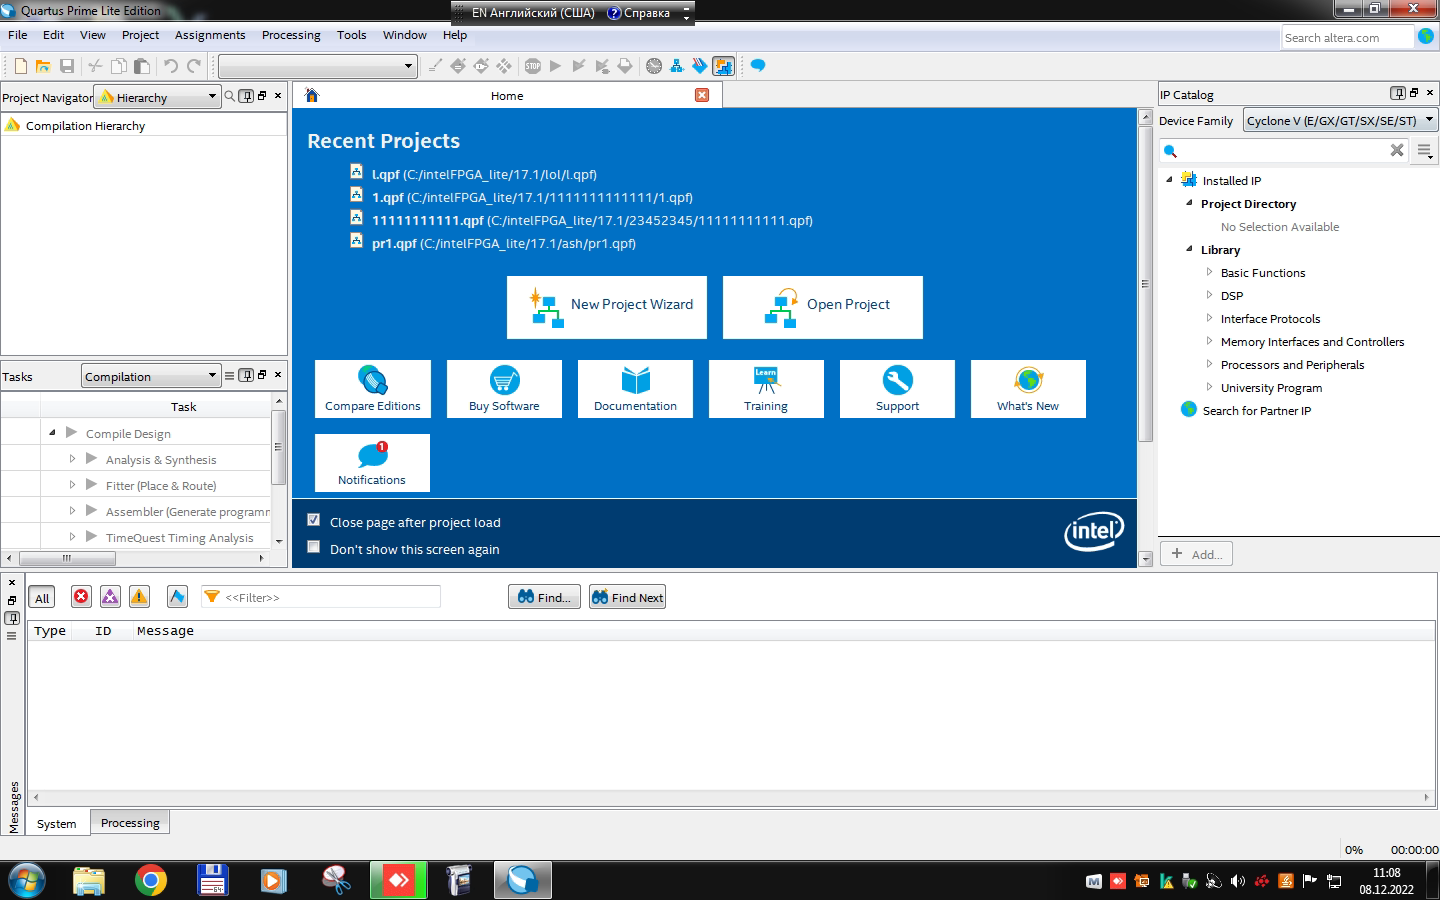
\includegraphics[width=0.95\textwidth]{02_01}
    \caption{открываем Quartus}
  \end{figure}

  \begin{figure}[H]
    \centering
    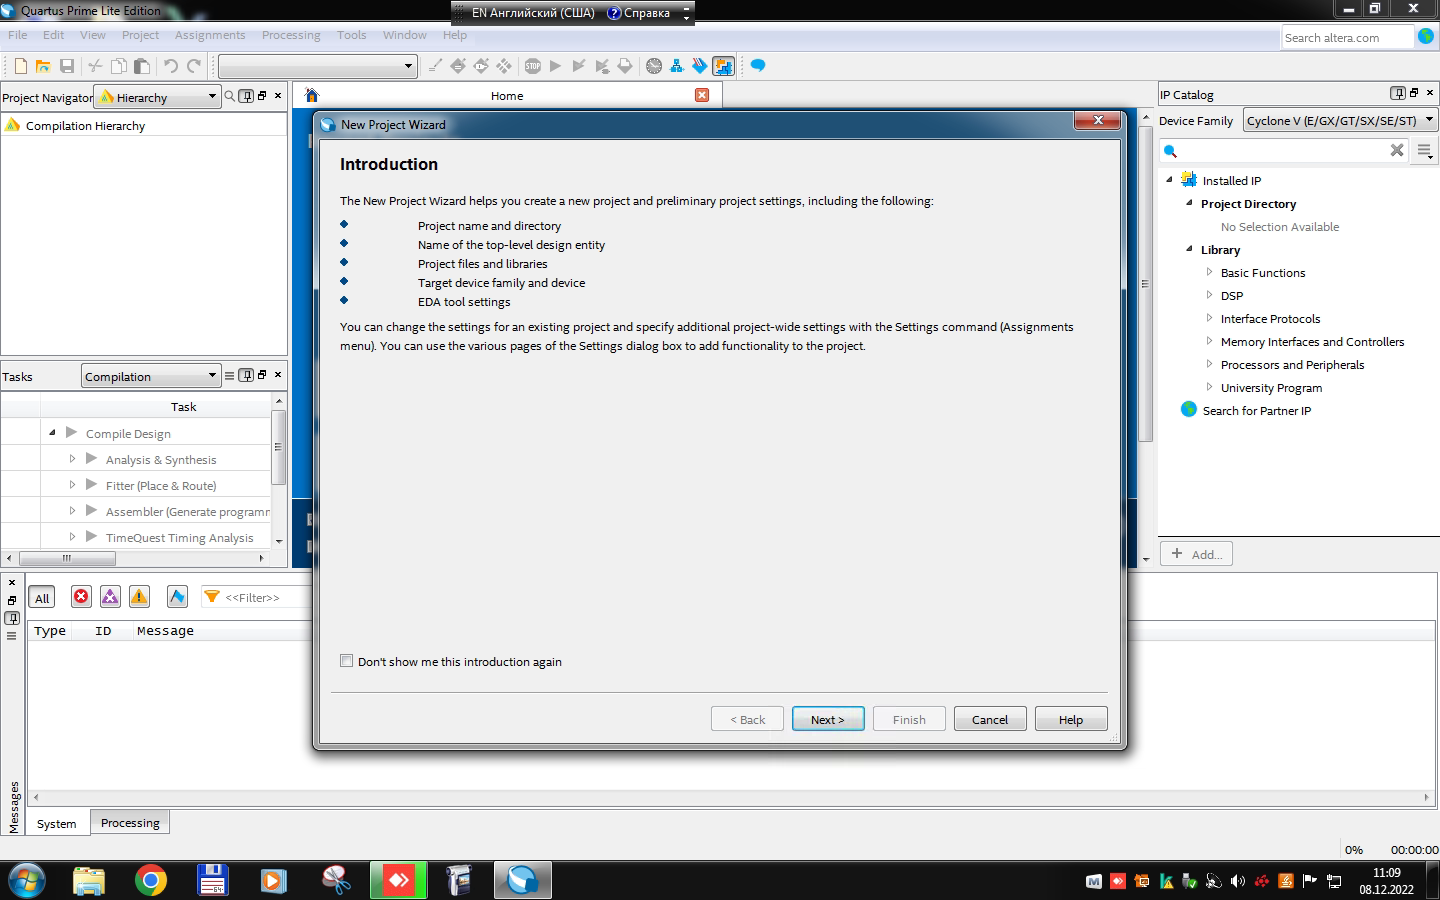
\includegraphics[width=0.95\textwidth]{02_02}
    \caption{начинаем создание нового проекта}
  \end{figure}

  \begin{figure}[H]
    \centering
    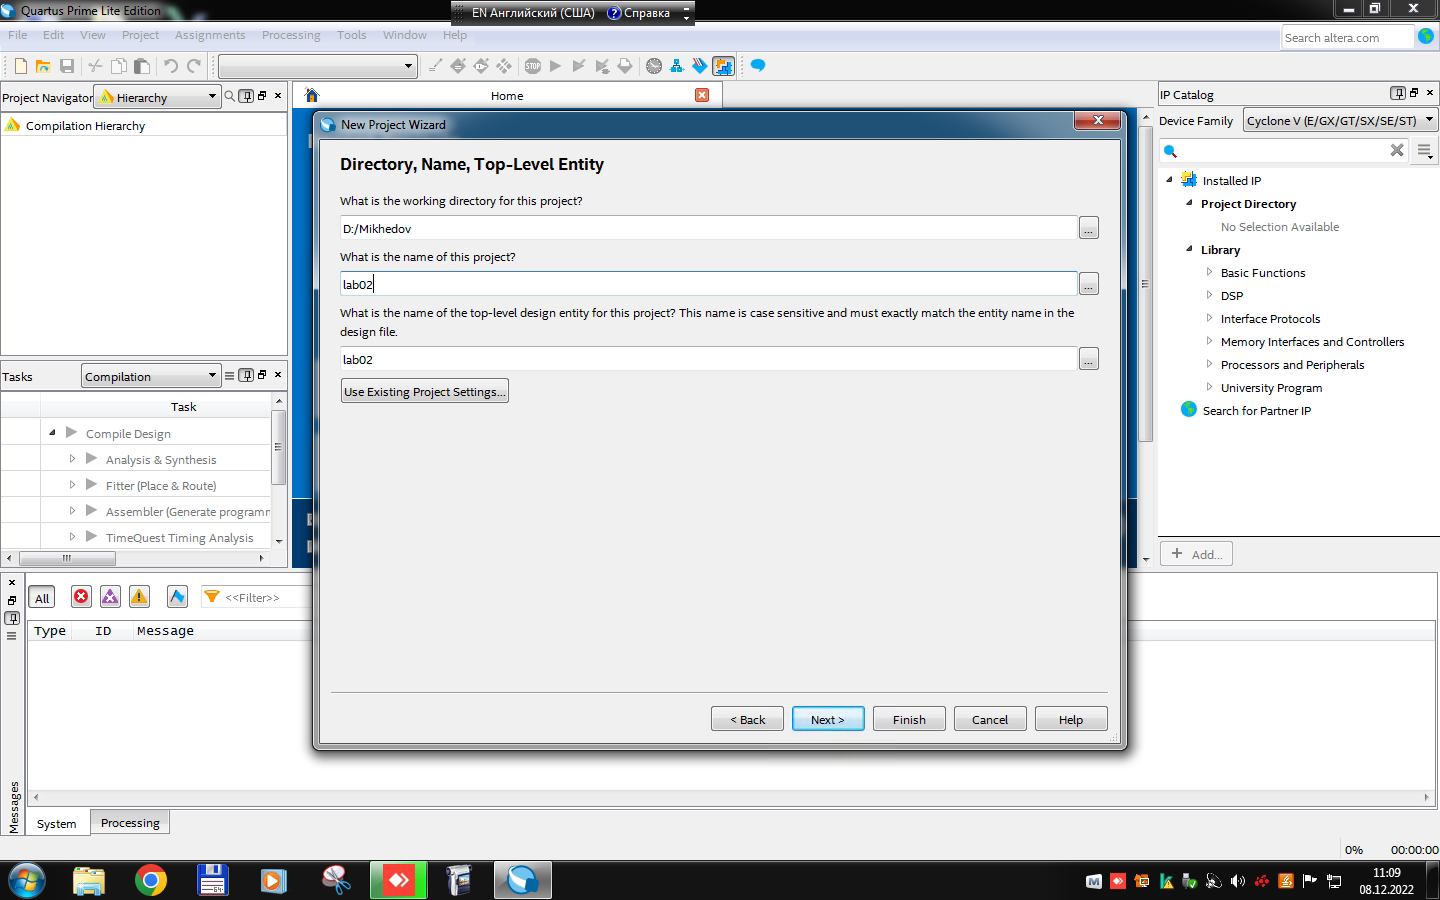
\includegraphics[width=0.95\textwidth]{02_03}
    \caption{выбираем расположение и имя проекта}
  \end{figure}

  \begin{figure}[H]
    \centering
    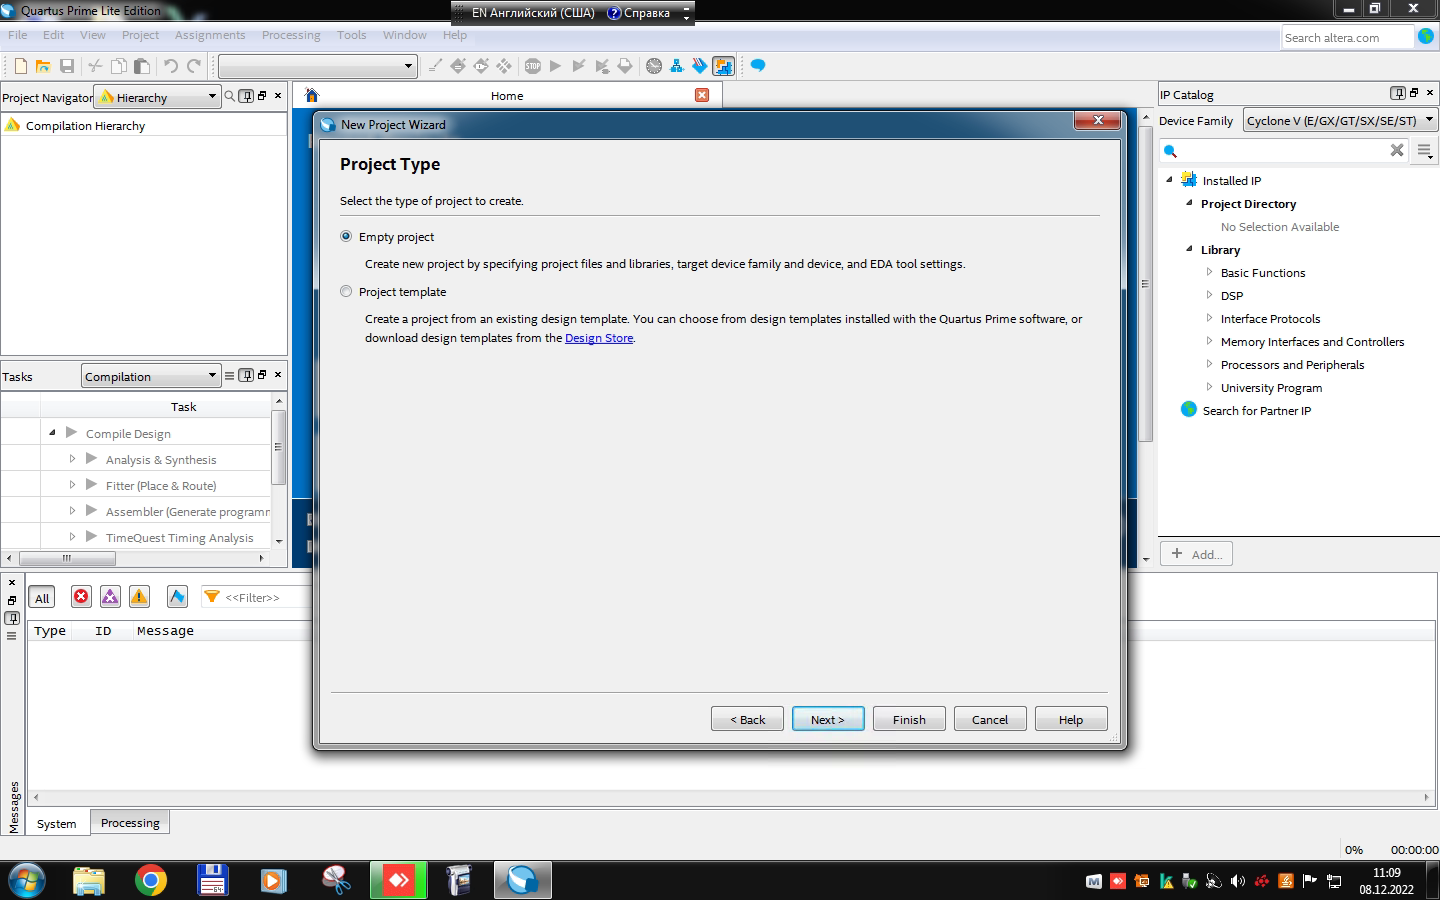
\includegraphics[width=0.95\textwidth]{02_04}
    \caption{пустой проект}
  \end{figure}

  \begin{figure}[H]
    \centering
    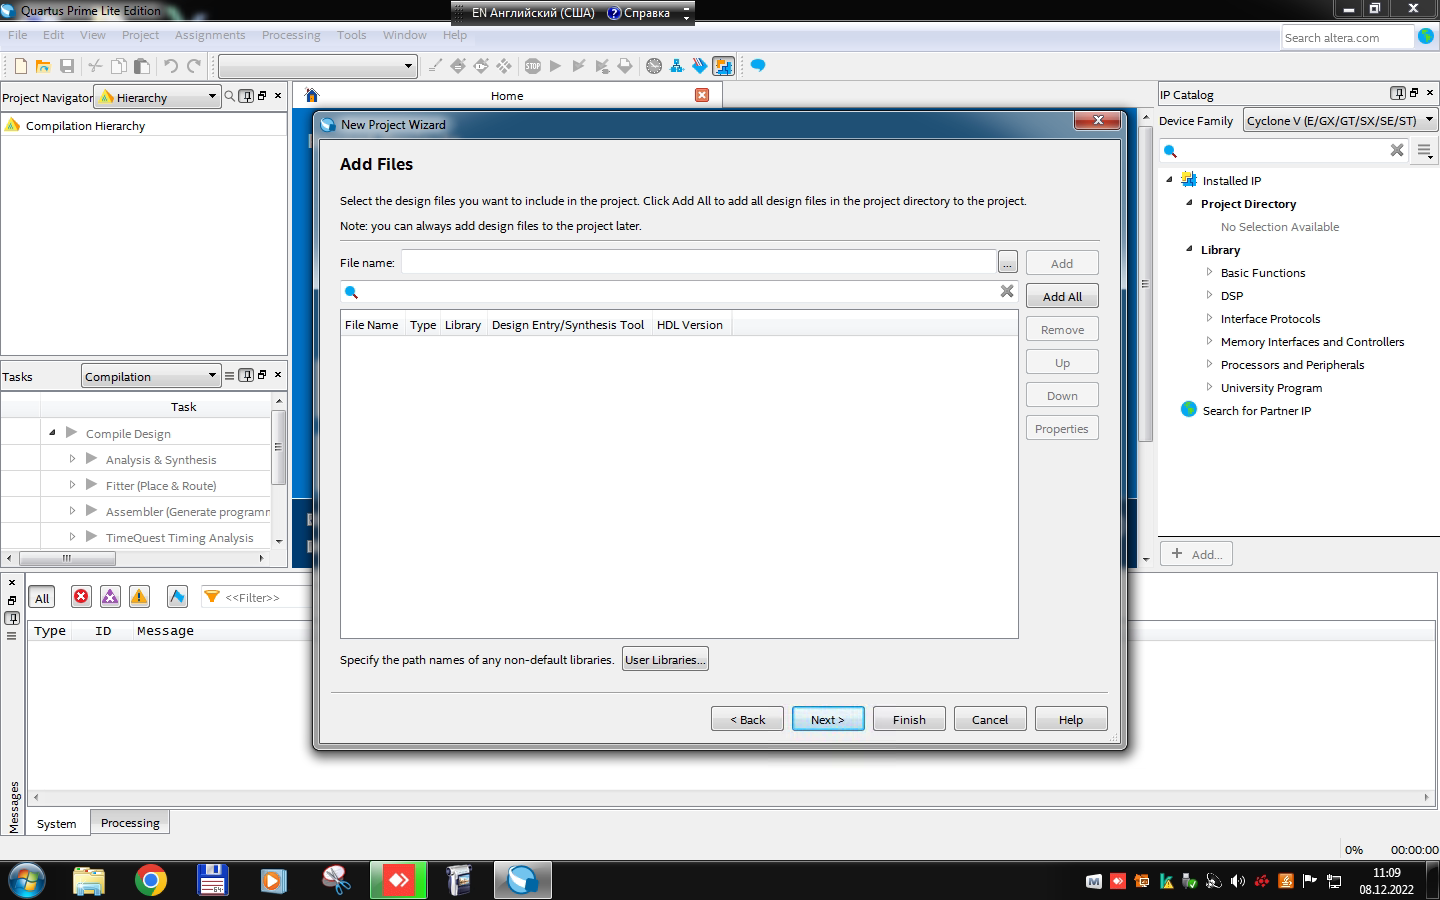
\includegraphics[width=0.95\textwidth]{02_05}
    \caption{проект без начальных файлов}
  \end{figure}

  \begin{figure}[H]
    \centering
    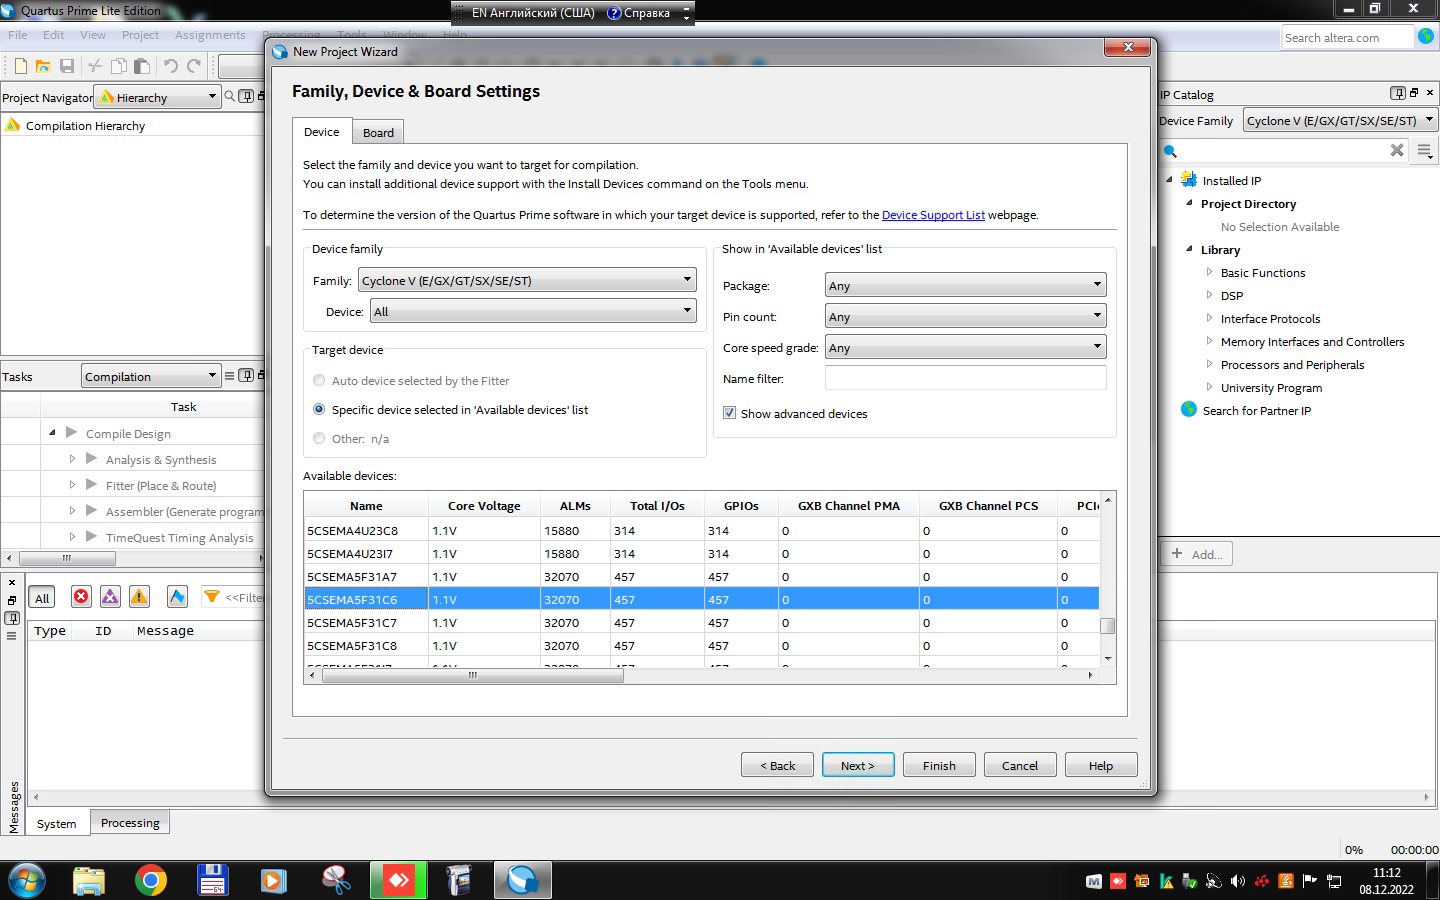
\includegraphics[width=0.95\textwidth]{02_06}
    \caption{выбираем необходимую плату}
  \end{figure}

  \begin{figure}[H]
    \centering
    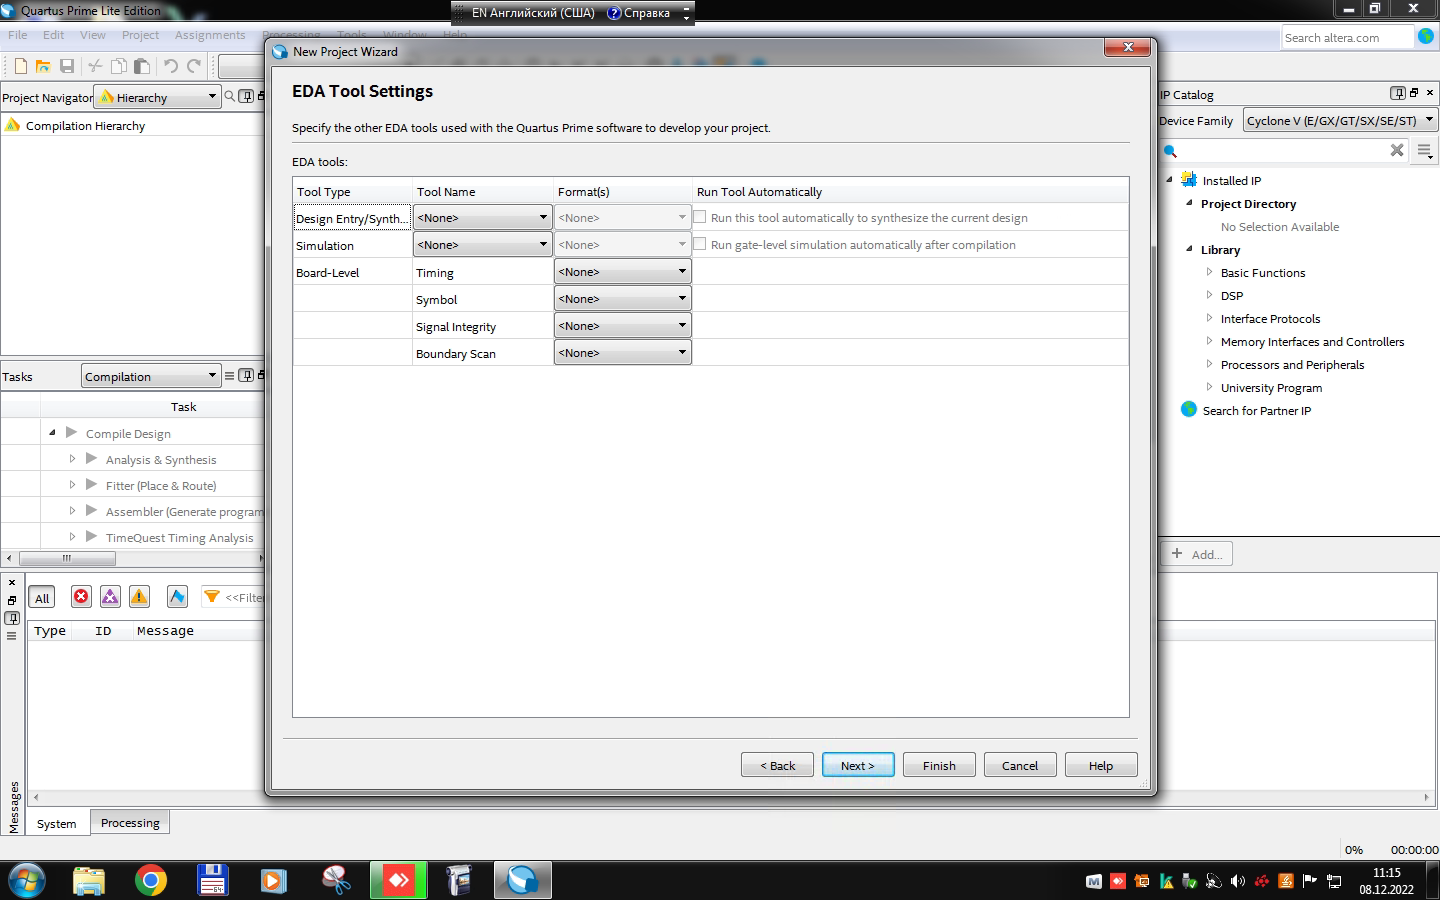
\includegraphics[width=0.95\textwidth]{02_07}
    \caption{дополнительные настройки}
  \end{figure}

  \begin{figure}[H]
    \centering
    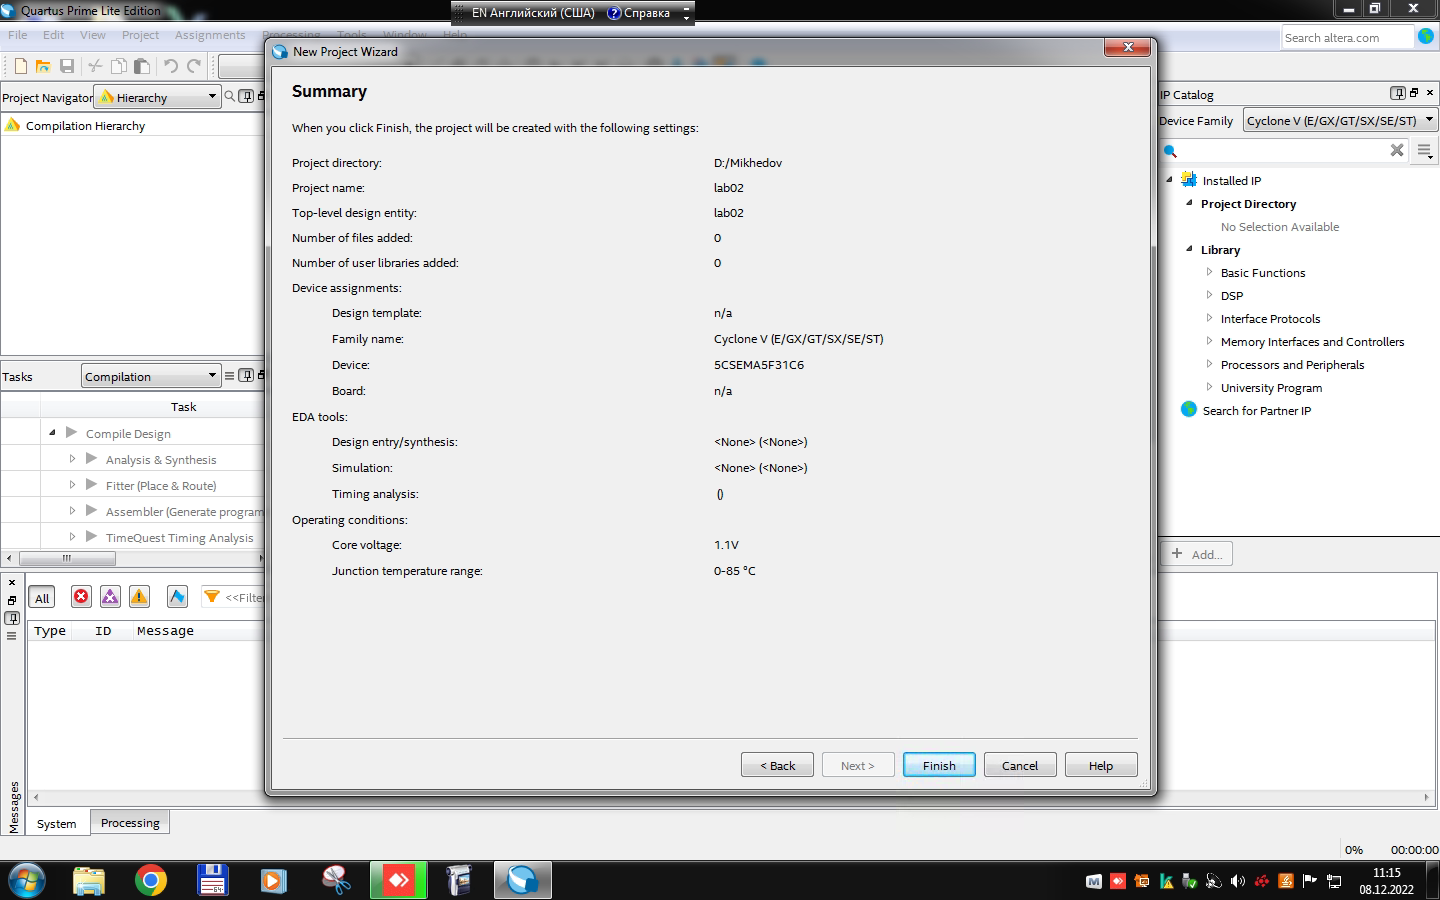
\includegraphics[width=0.95\textwidth]{02_08}
    \caption{проект создан}
  \end{figure}

  Далее нужно построить СКНФ и СДНФ при помощи логических элементов:

  \begin{figure}[H]
    \centering
    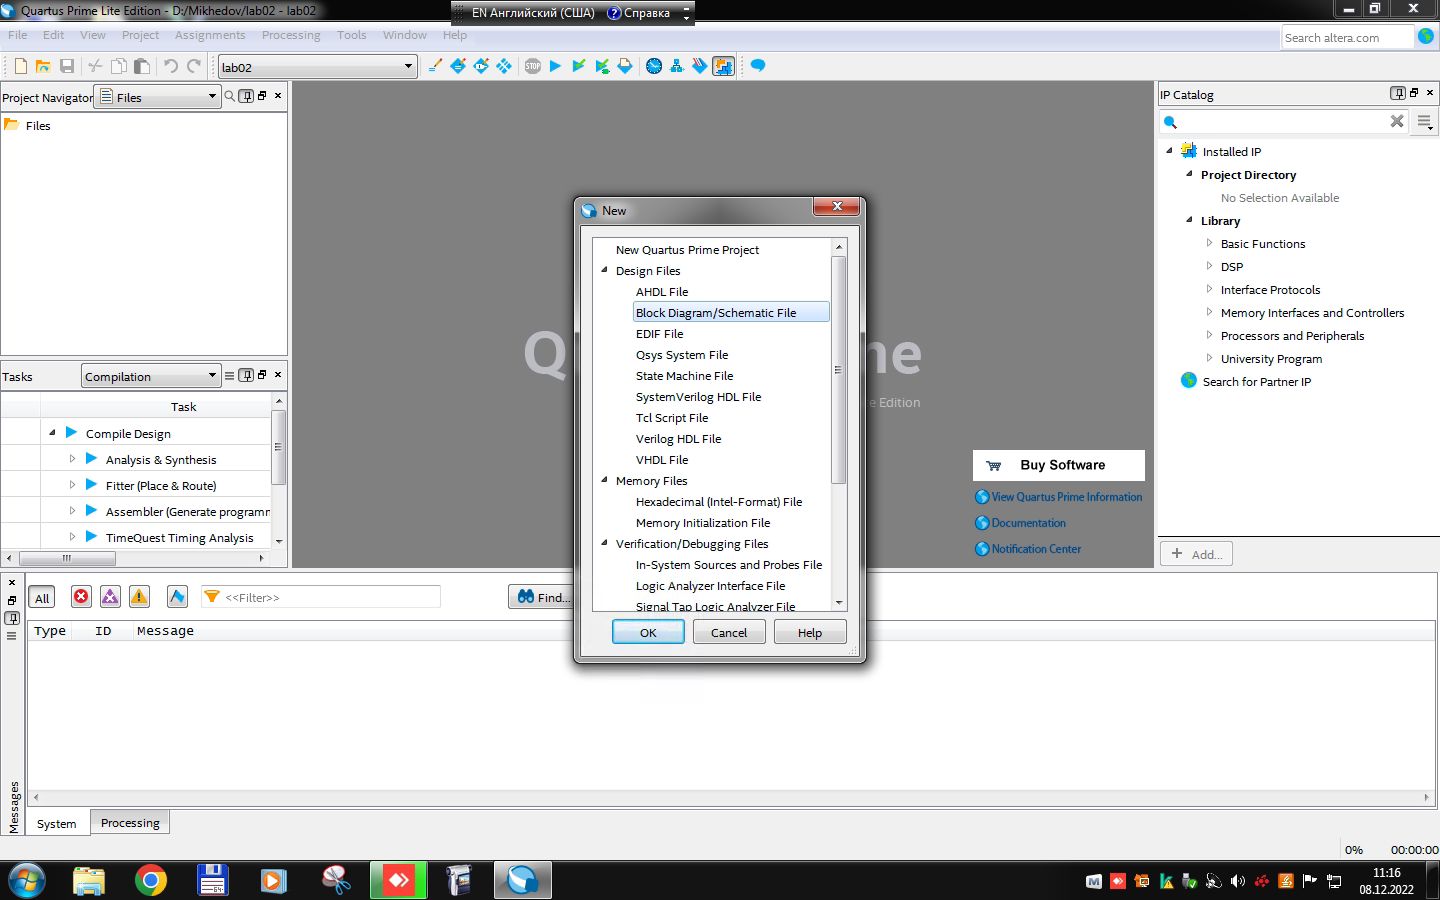
\includegraphics[width=0.93\textwidth]{02_10}
    \caption{создаем новый файл схемы}
  \end{figure}
  
  \begin{figure}[H]
    \centering
    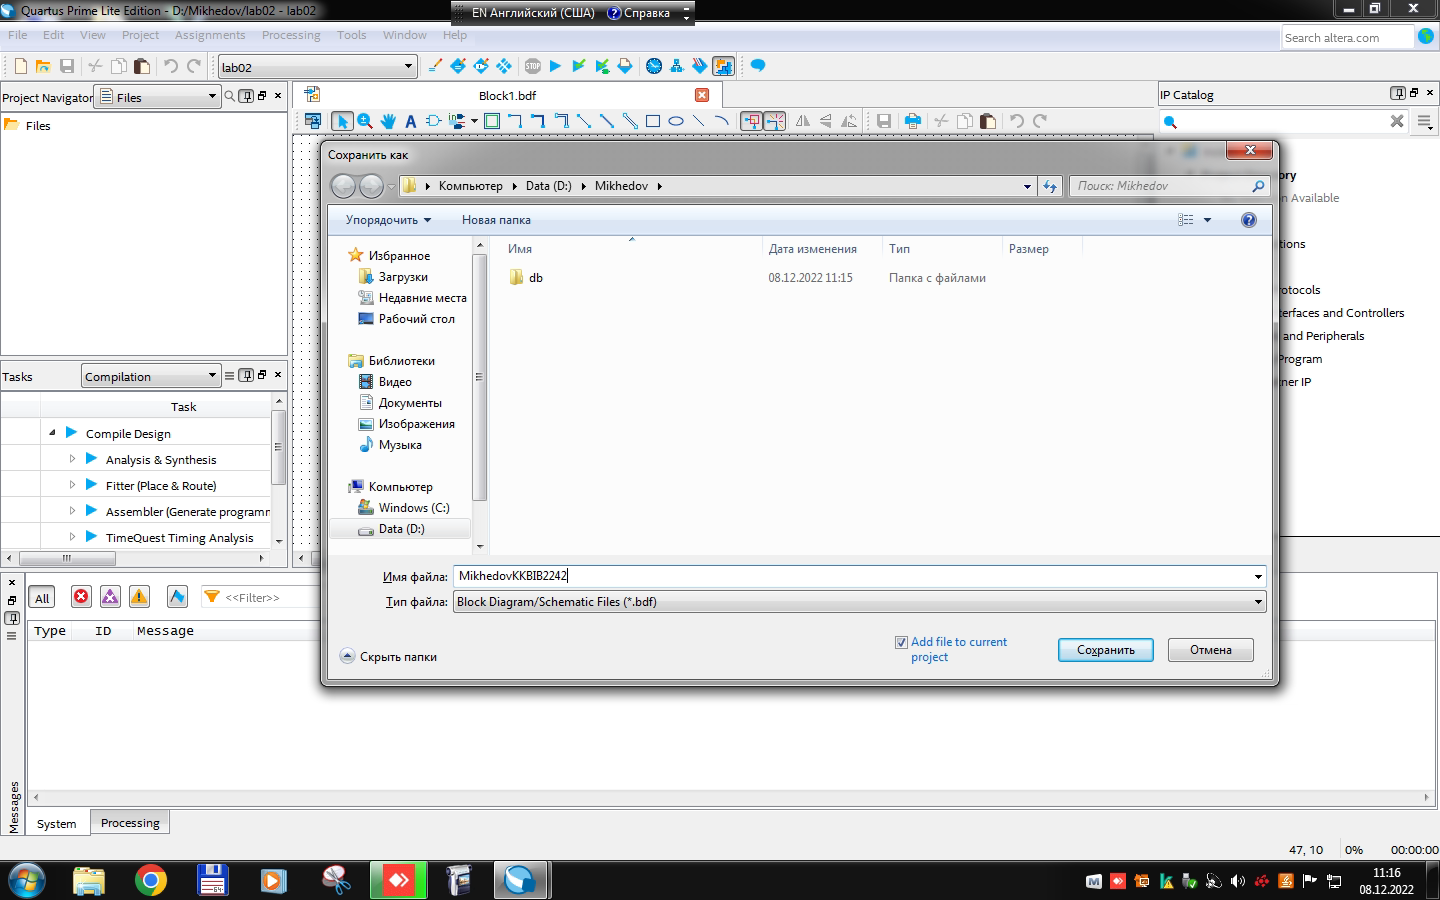
\includegraphics[width=0.93\textwidth]{02_11}
    \caption{назначаем ему имя}
  \end{figure}
  
  \begin{figure}[H]
    \centering
    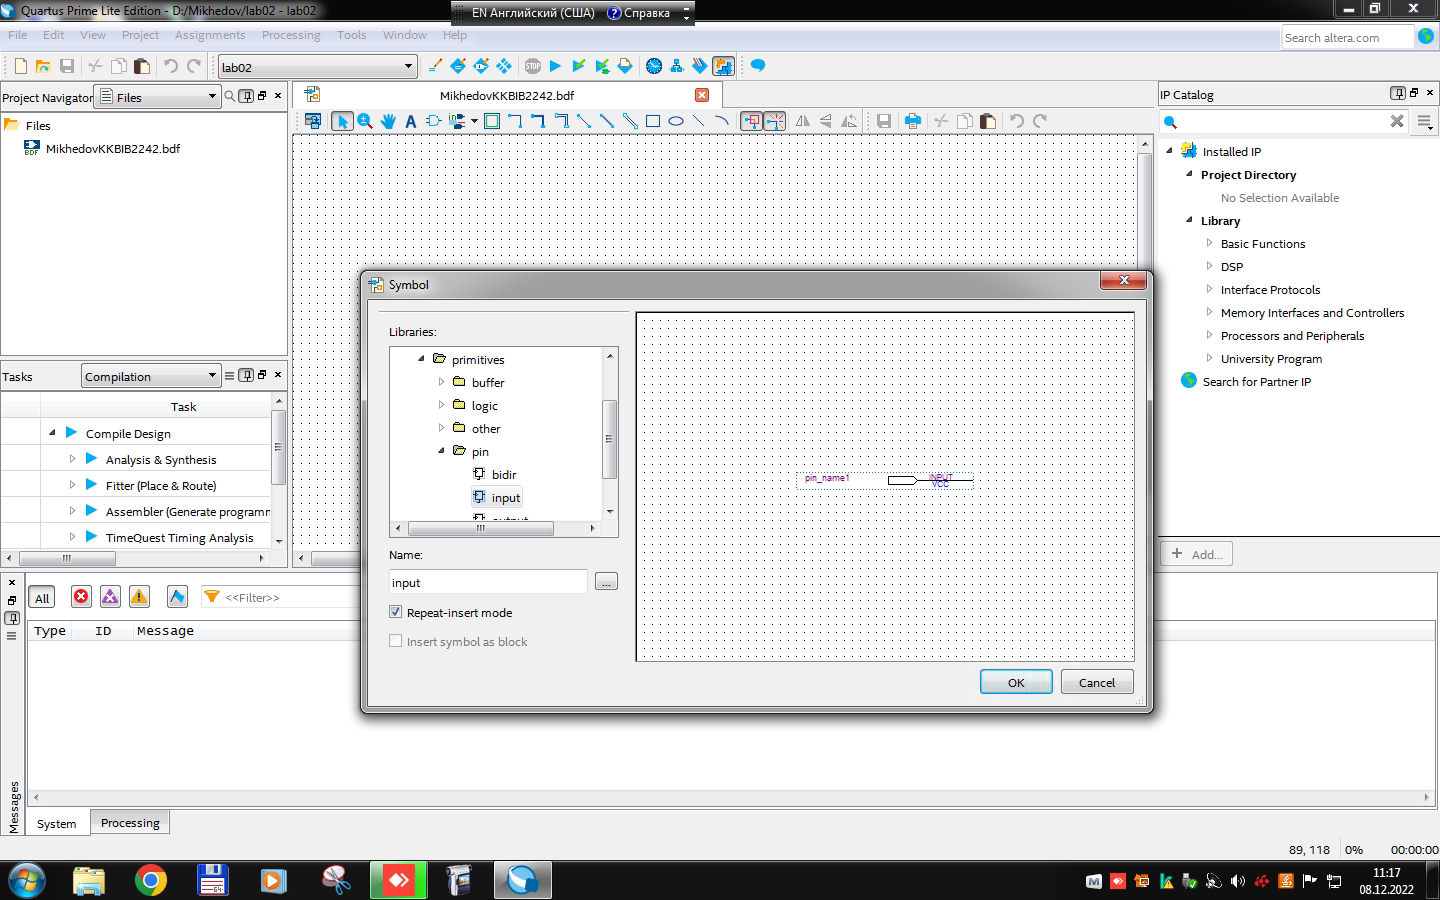
\includegraphics[width=0.9475\textwidth]{02_12}
    \caption{добавляем входы и выходы}
  \end{figure}
  
  \begin{figure}[H]
    \centering
    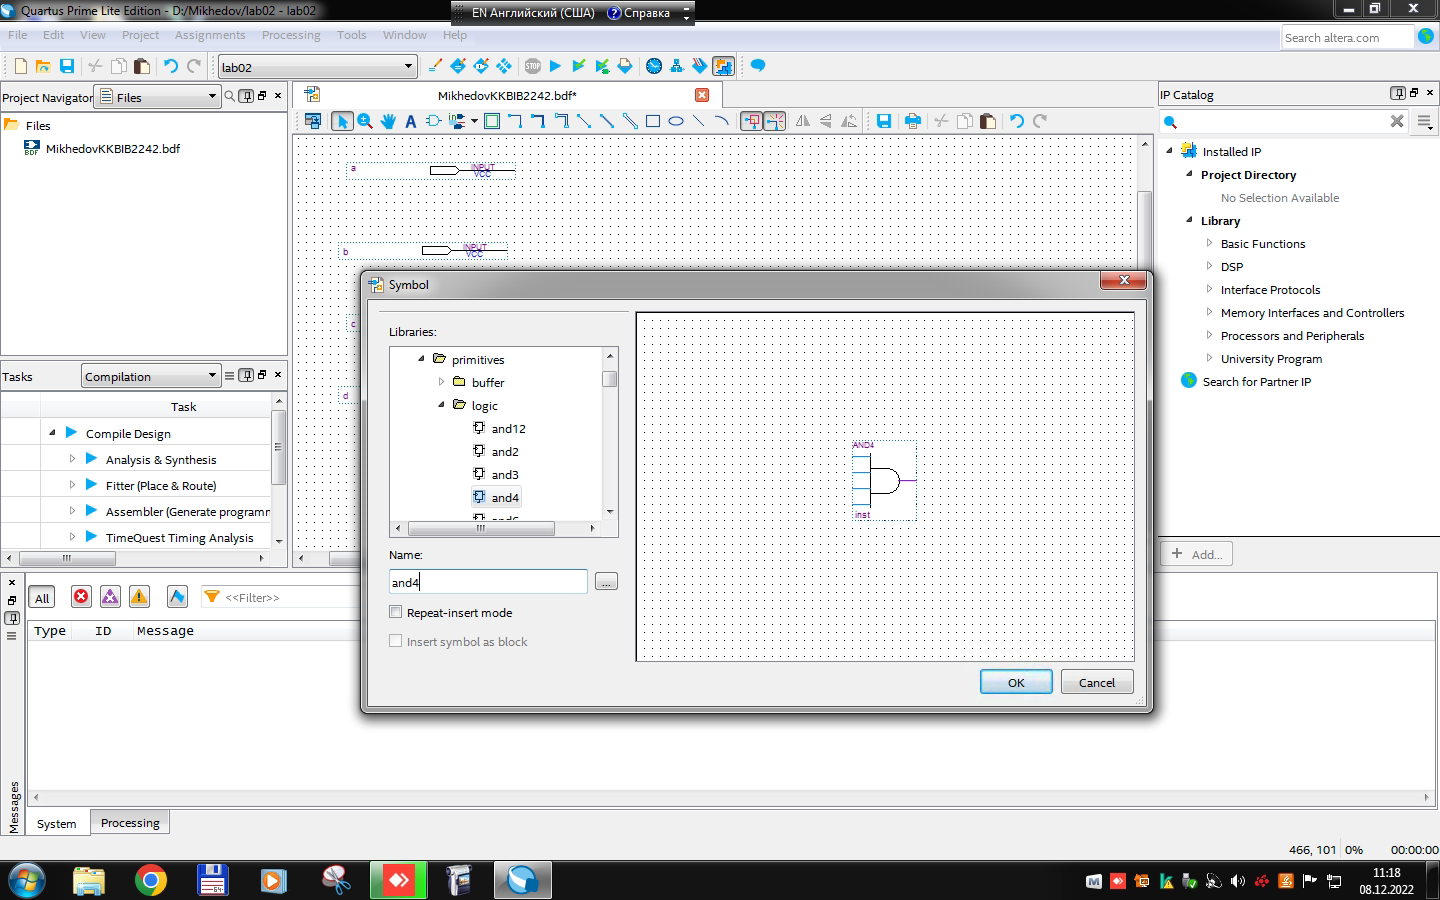
\includegraphics[width=0.9475\textwidth]{02_13}
    \caption{добавляем логические элементы}
  \end{figure}
  
  \begin{figure}[H]
    \centering
    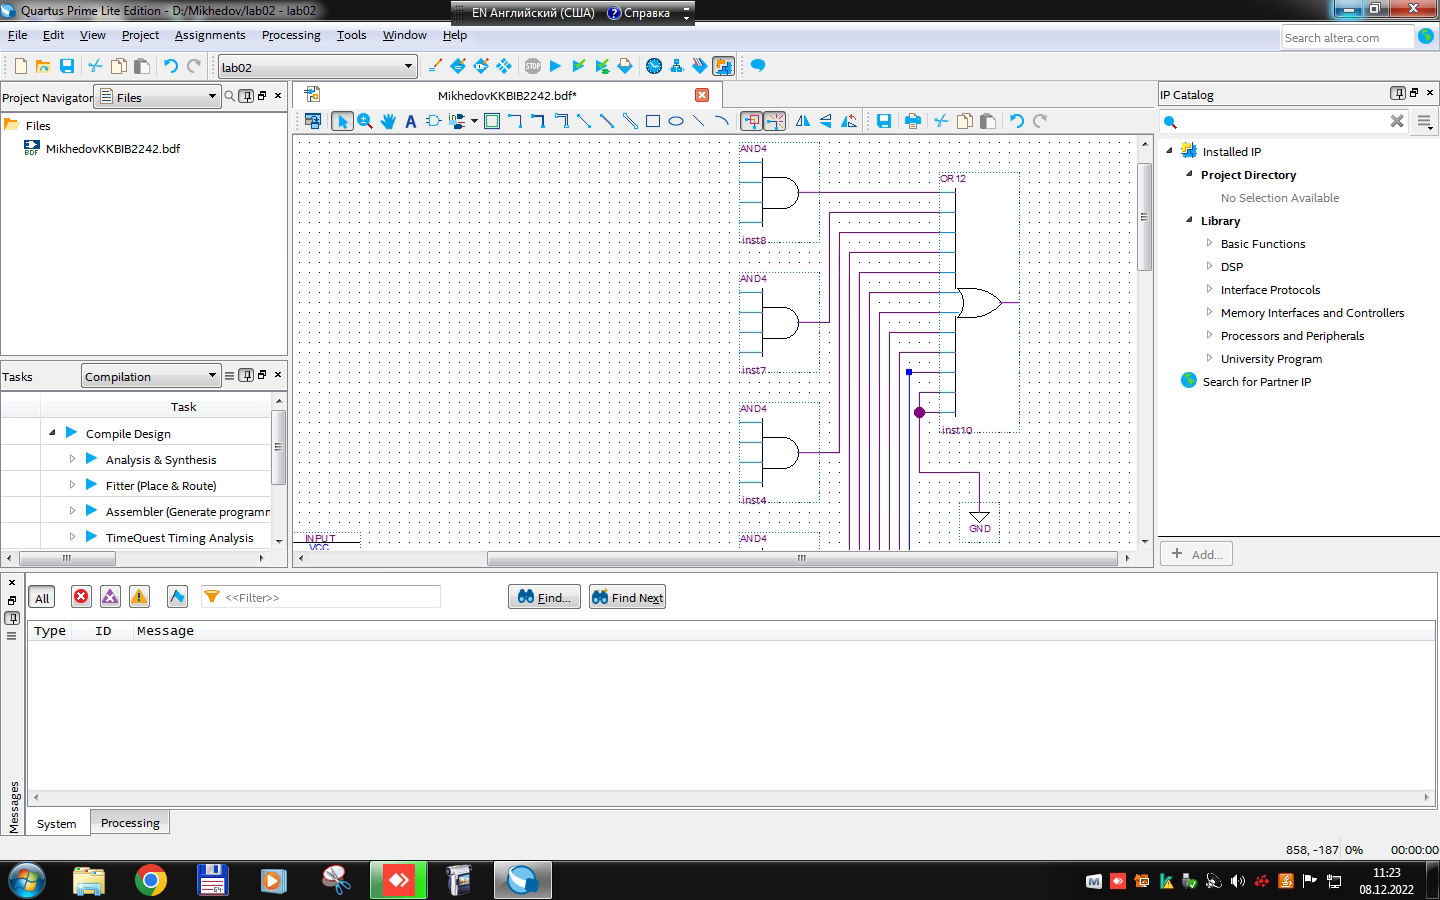
\includegraphics[width=0.9475\textwidth]{02_14}
    \caption{построение СДНФ}
  \end{figure}
  
  \begin{figure}[H]
    \centering
    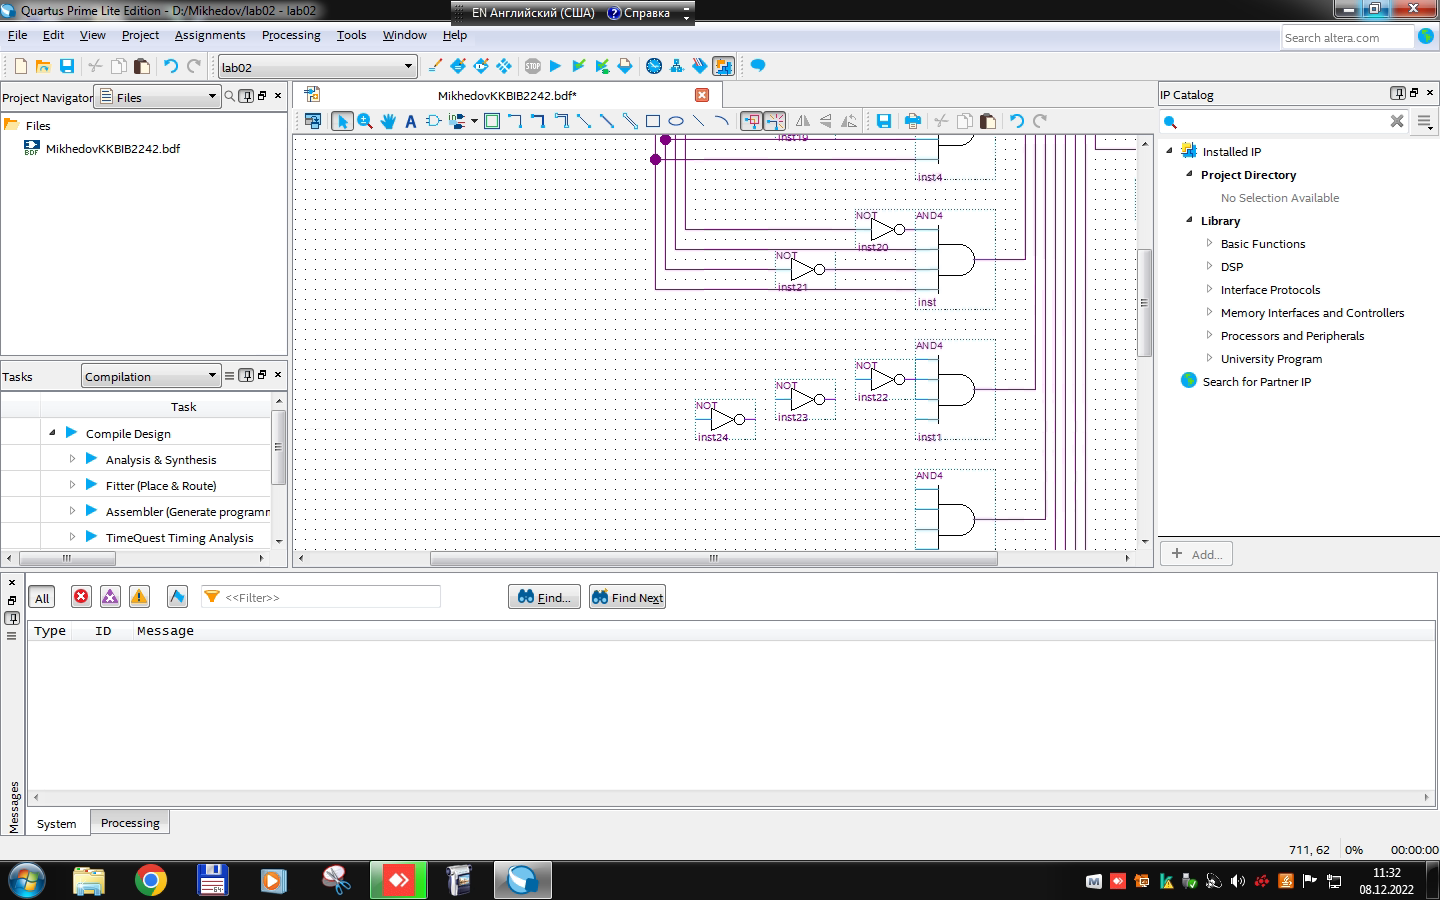
\includegraphics[width=0.9475\textwidth]{02_15}
    \caption{построение СДНФ}
  \end{figure}
  
  \begin{figure}[H]
    \centering
    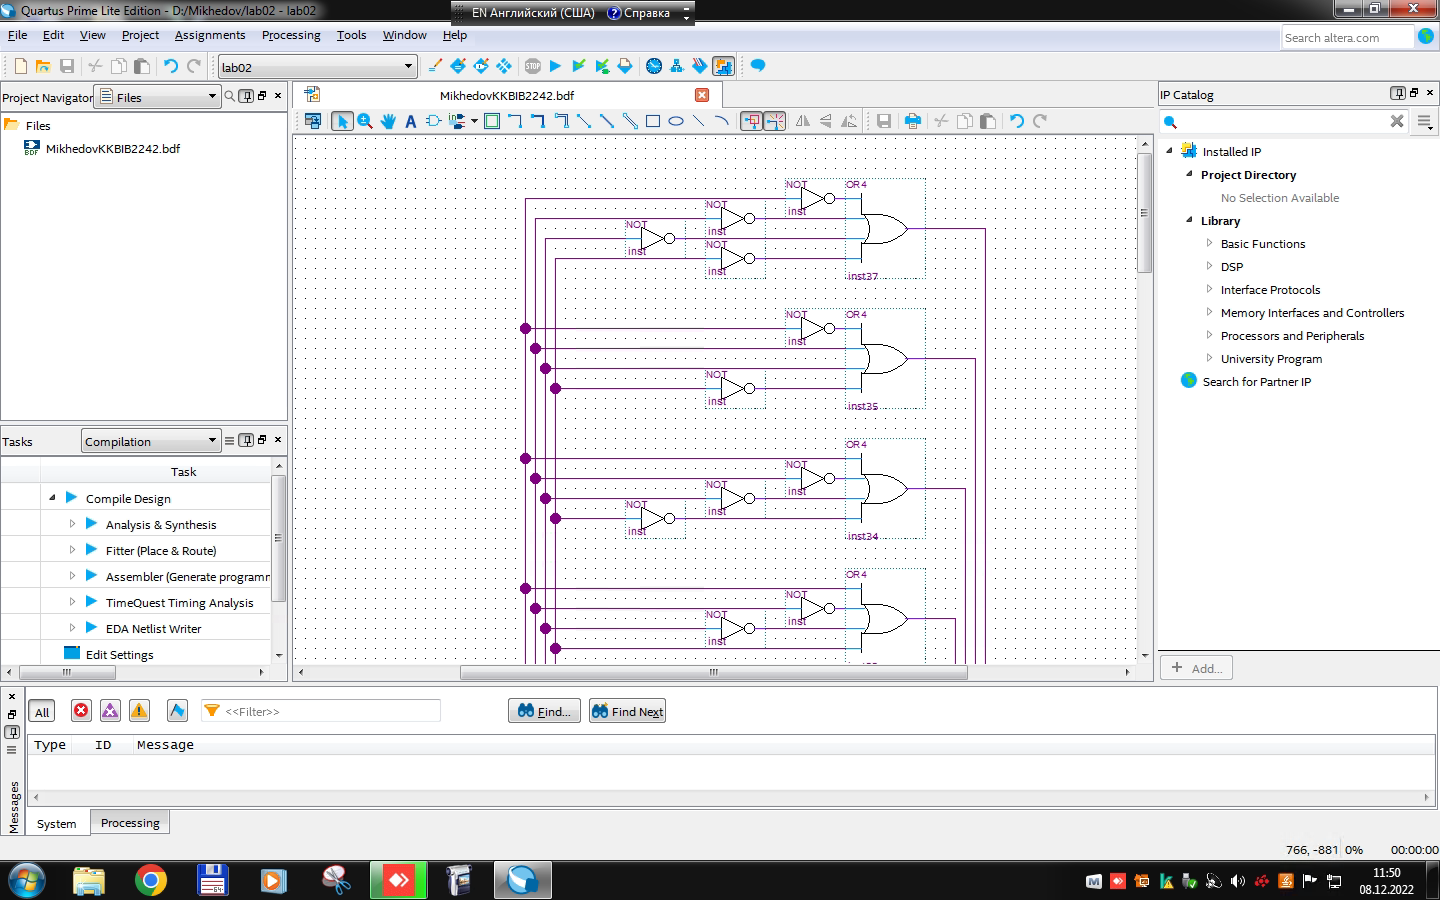
\includegraphics[width=0.9475\textwidth]{02_16}
    \caption{построение СКНФ}
  \end{figure}
  
  \begin{figure}[H]
    \centering
    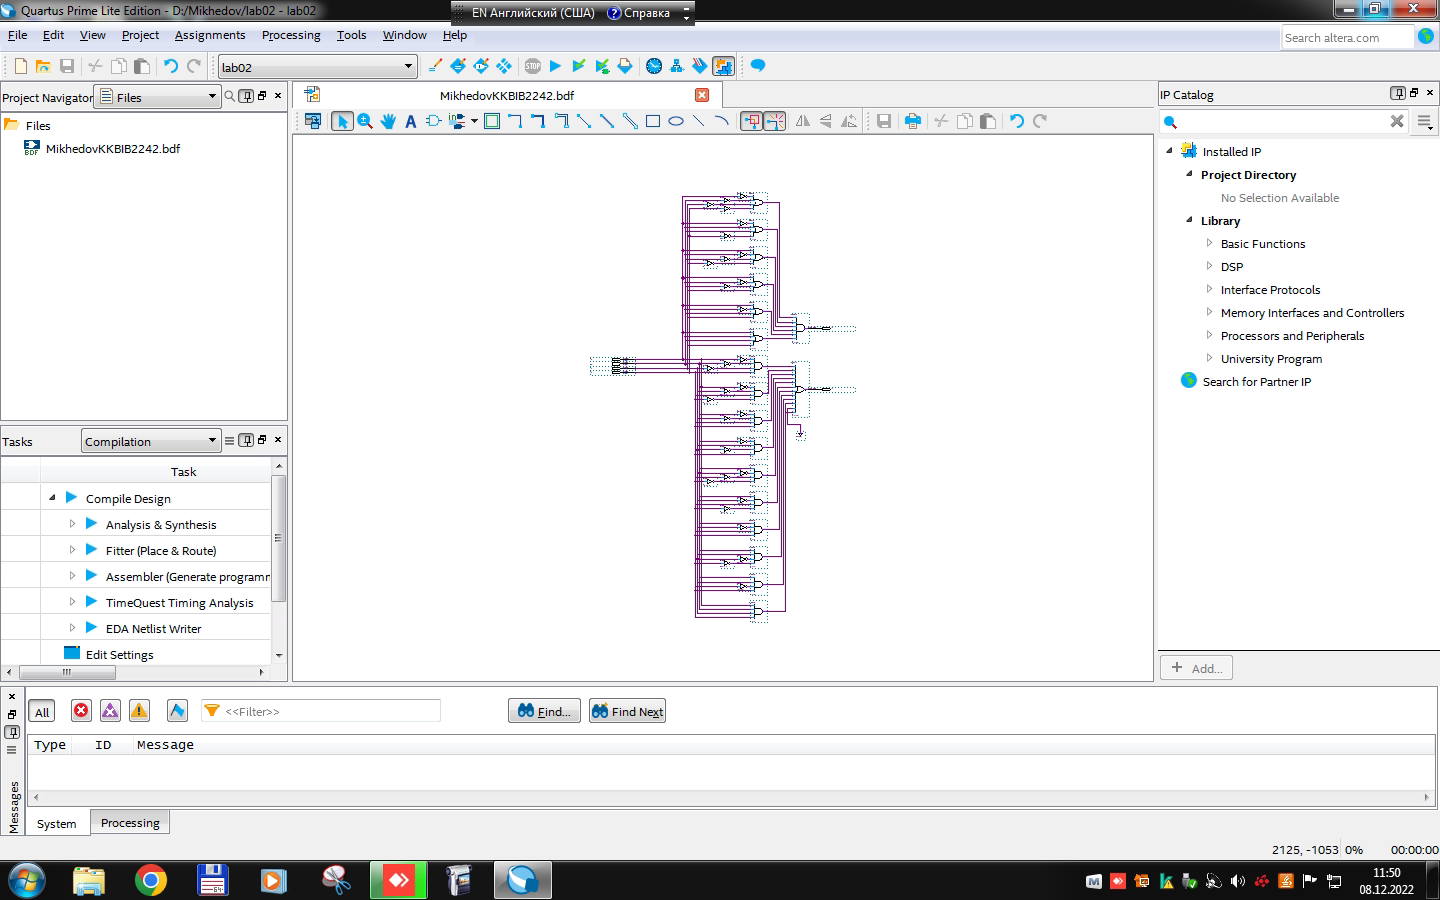
\includegraphics[width=0.9475\textwidth]{02_17}
    \caption{построенная схема (СДНФ и СКНФ)}
  \end{figure}
  
  Теперь нужно запустить функциональную симуляцию:

  \begin{figure}[H]
    \centering
    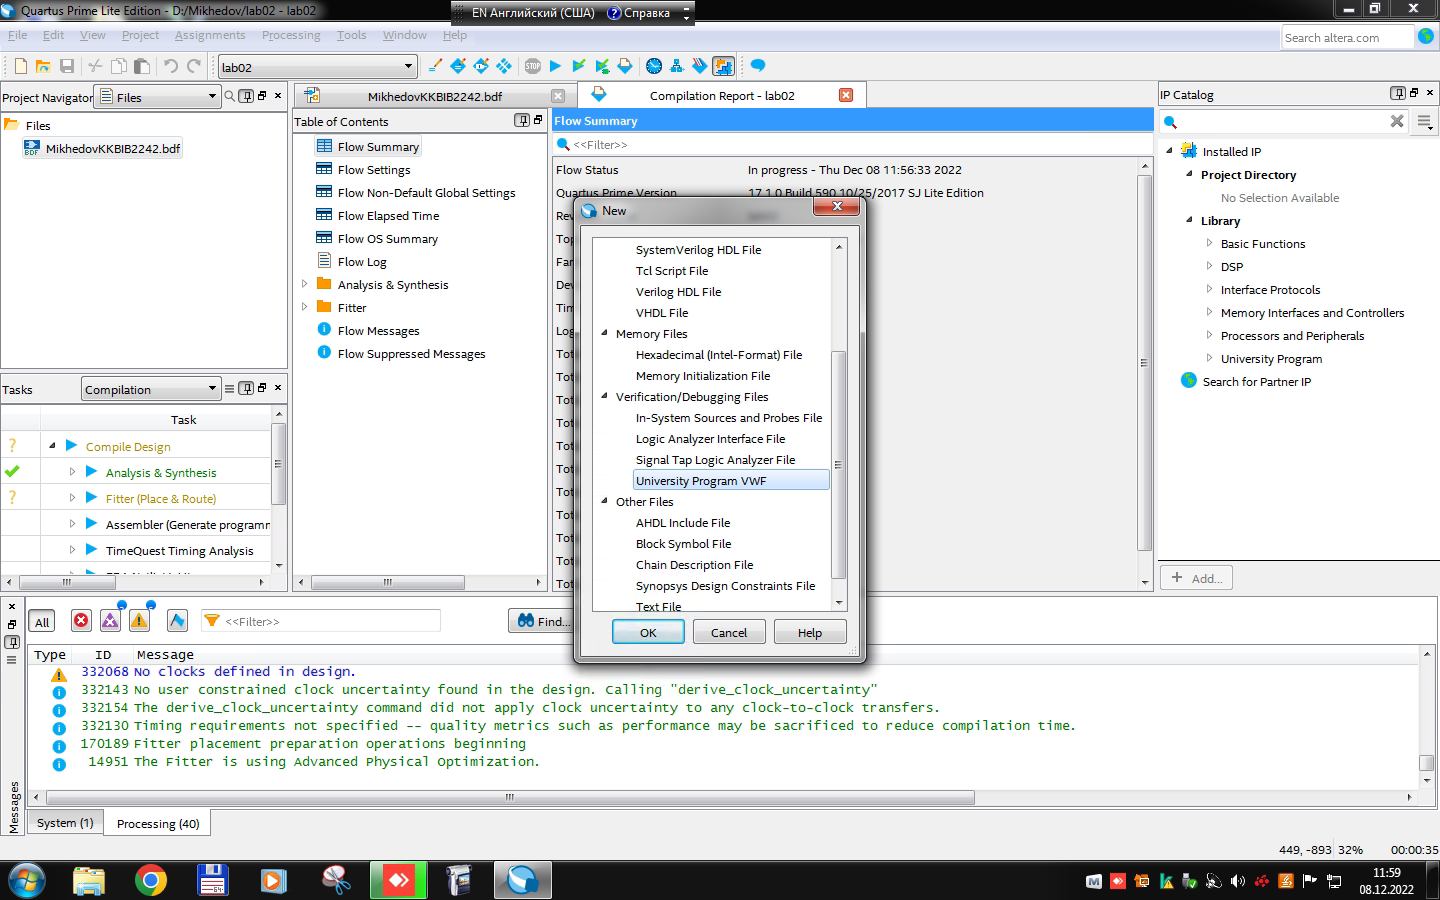
\includegraphics[width=0.93\textwidth]{02_31}
    \caption{создаем новый wvf-файл}
  \end{figure}

  \begin{figure}[H]
    \centering
    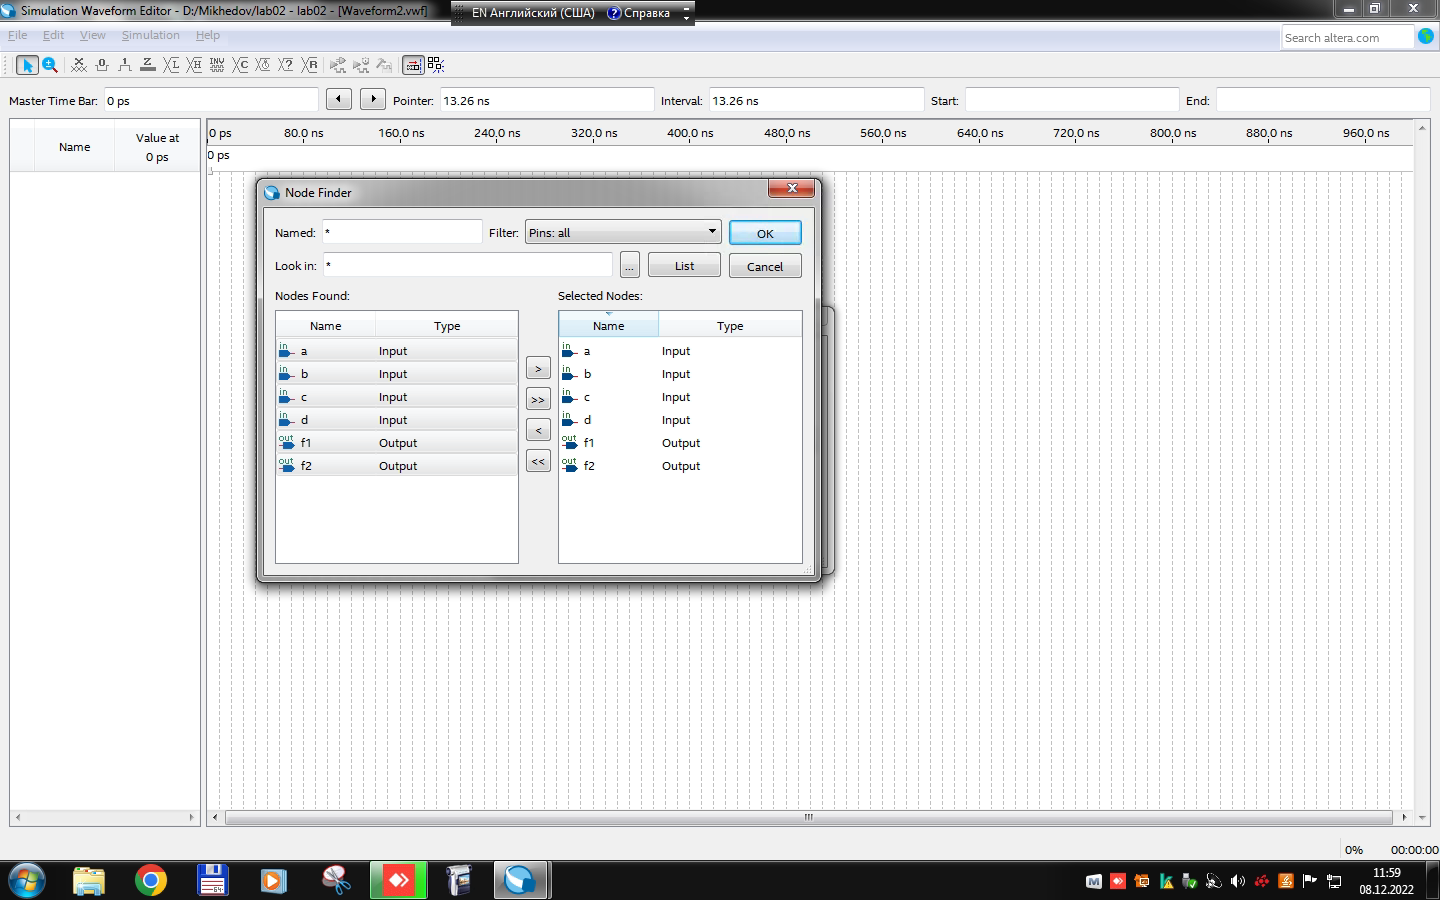
\includegraphics[width=0.93\textwidth]{02_32}
    \caption{добавляем все входы и выходы}
  \end{figure}

  \begin{figure}[H]
    \centering
    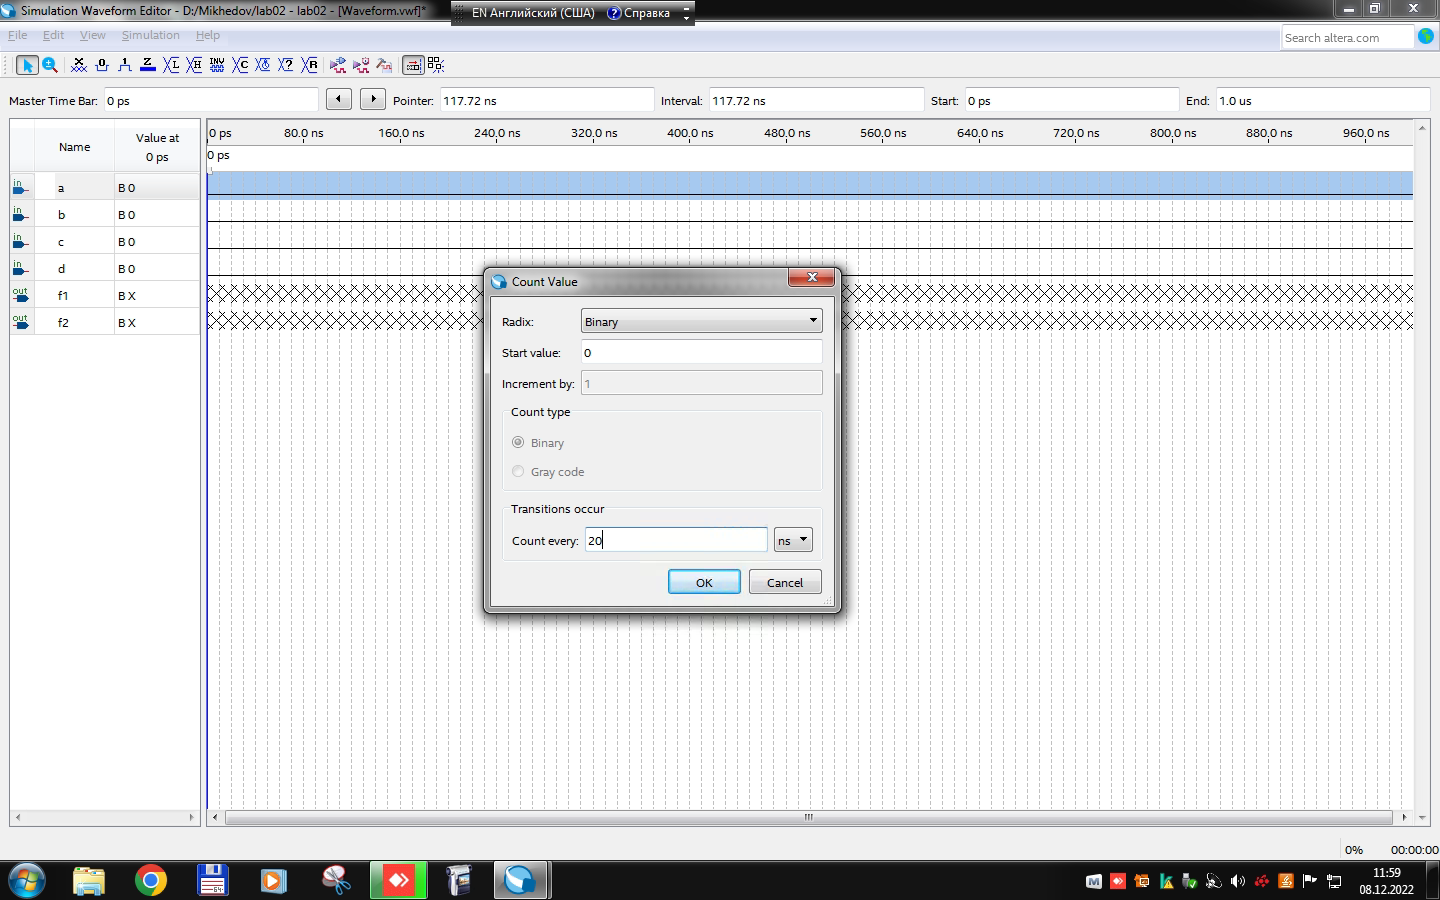
\includegraphics[width=0.9475\textwidth]{02_33}
    \caption{устанавливаем значения на входах}
  \end{figure}

  \begin{figure}[H]
    \centering
    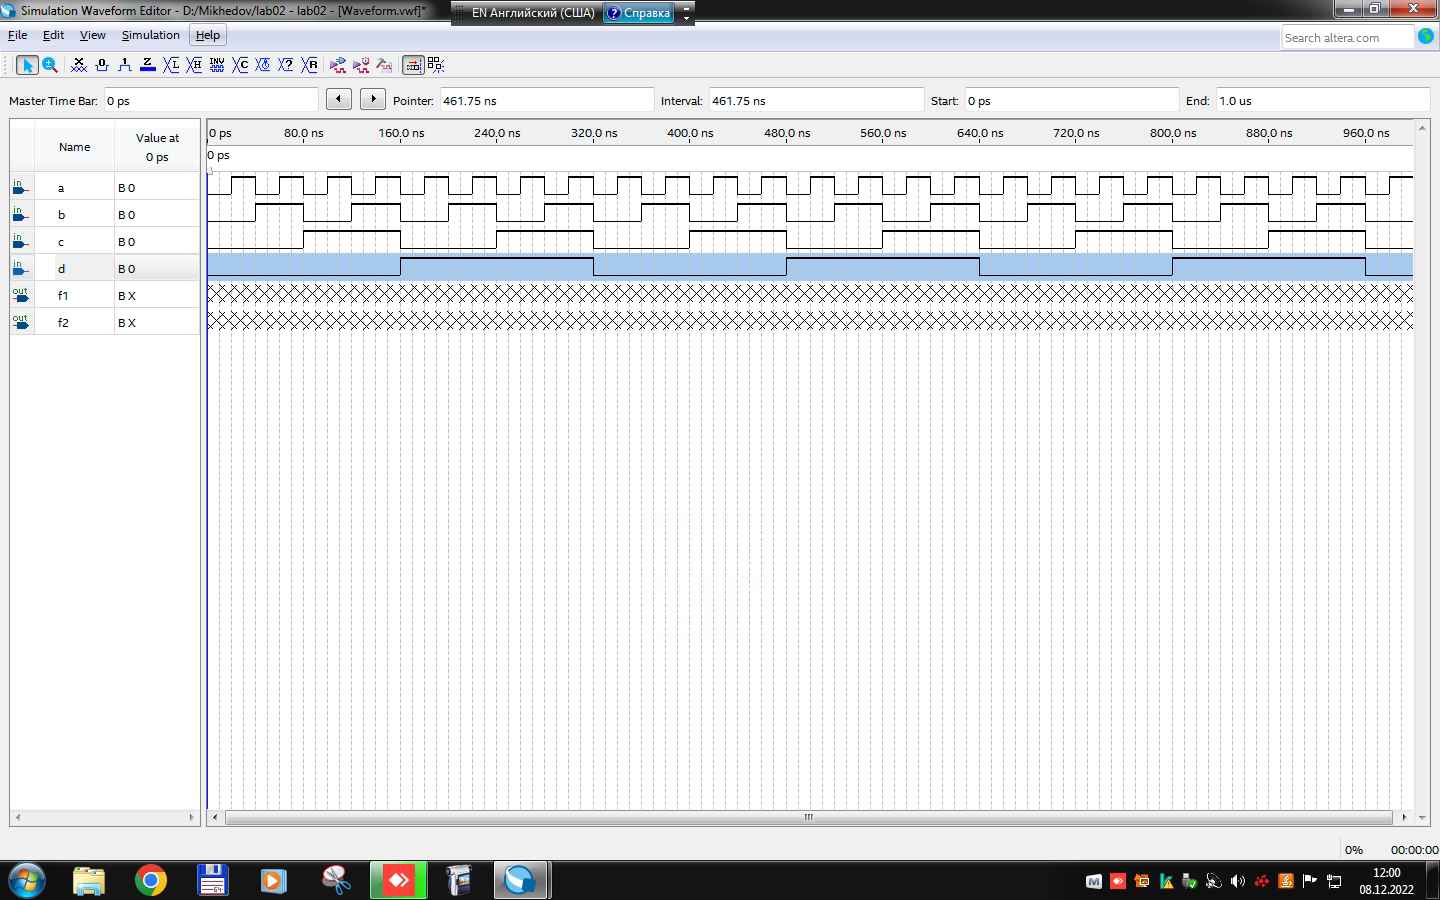
\includegraphics[width=0.9475\textwidth]{02_34}
    \caption{полученные значения для входов}
  \end{figure}

  \begin{figure}[H]
    \centering
    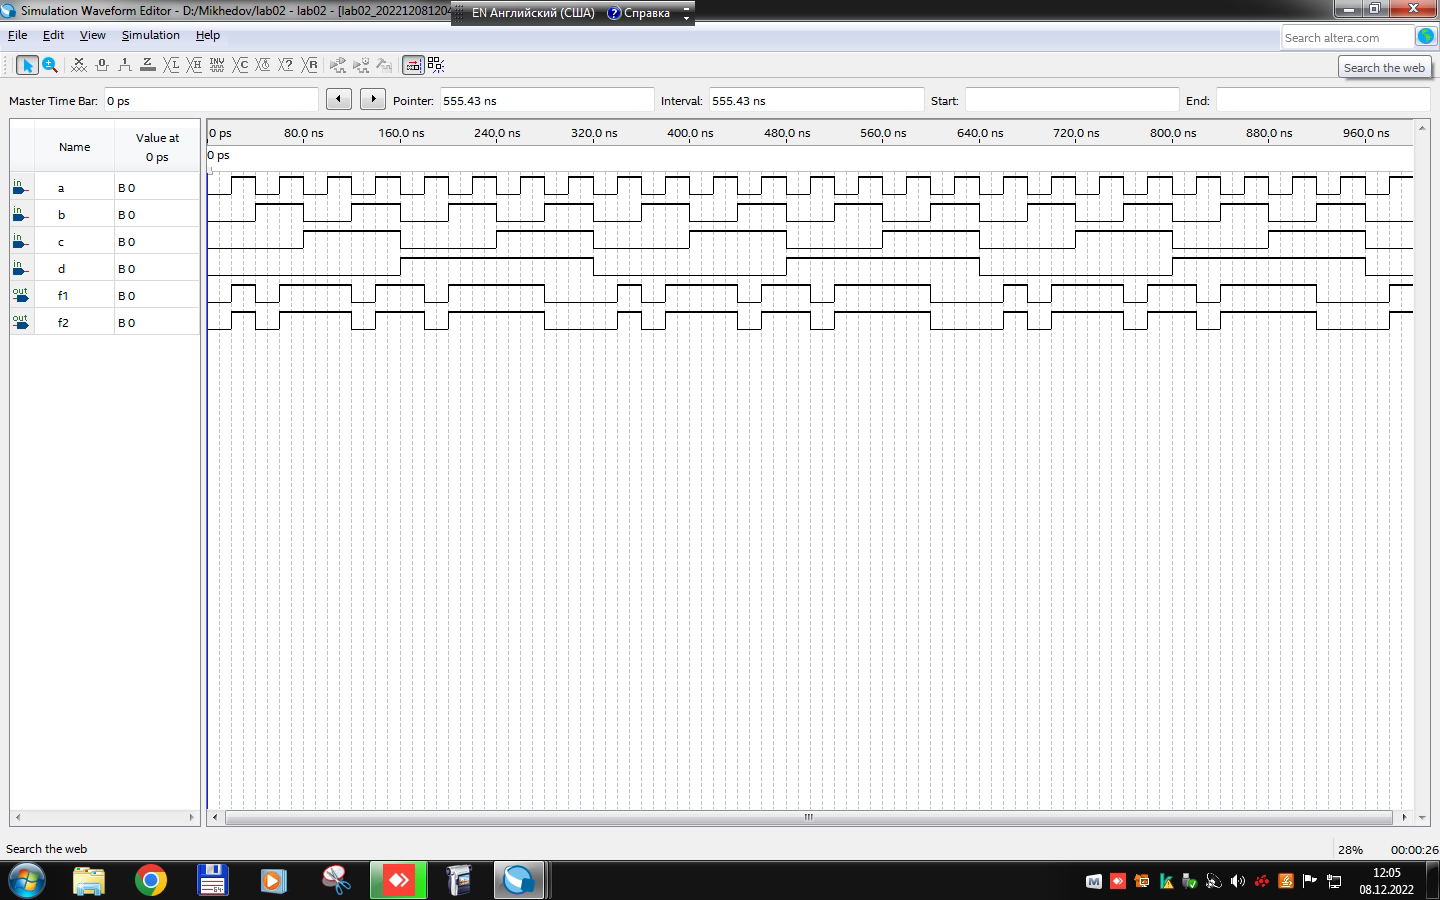
\includegraphics[width=0.9475\textwidth]{02_30}
    \caption{результат функциональной симуляции}
  \end{figure}

  Видно, что схема СКНФ и схема СДНФ дают одинаковый с таблицей истинности результат.

  \section*{Пункт 2}

  Выполним минимизацию исходного выражения при помощи метода Квайна-Мак-Класки. Для этого
  выполним все возможные склейки (таблица \ref{table:t2} на стр. \pageref{table:t2})

  \begin{table}[H]
    \centering
    \begin{tabular}{| c | c | c | c | c | c |}
      \hline
      \multicolumn{2}{| c |}{Этап 1} &
      \multicolumn{2}{| c |}{Этап 2} &
      \multicolumn{2}{| c |}{Этап 3} \\
      \hline
      $№$ & Минтерм & $№$ & Минтерм & $№$ & Минтерм \\
      \hline
      1 & $\overline{a}\overline{b}\overline{c}d$ &
      (1 - 3) & $\overline{a}\overline{b}d$ &
      (1 - 3) & $\overline{a}\overline{b}d$\\
      \hline
      2 & $\overline{a}\overline{b}c\overline{d}$ &
      (1 - 4) & $\overline{a}\overline{c}d$ &
      (1 - 4) & $\overline{a}\overline{c}d$ \\
      \hline
      3 & $\overline{a}\overline{b}cd$ &
      (2 - 3) & $\overline{a}\overline{b}c$ &
      ((2-3) - (6-7)) & $\overline{b}c$\\
      \hline
      4 & $\overline{a}b\overline{c}d$ &
      (2 - 6) & $\overline{b}c\overline{d}$ &
      ((2-6) - (3-7)) & $\overline{b}c$\\
      \hline
      5 & $a\overline{b}\overline{c}\overline{d}$ &
      (3 - 7) & $\overline{b}cd$ &
      (4 - 9) & $b\overline{c}d$ \\
      \hline
      6 & $a\overline{b}c\overline{d}$ &
      (4 - 9) & $b\overline{c}d$ &
      ((5-6) - (8-10)) & $a\overline{d}$ \\
      \hline
      7 & $a\overline{b}cd$ &
      (5 - 6) & $a\overline{b}\overline{d}$ &
      ((5-8) - (6-10)) & $a\overline{d}$ \\
      \hline
      8 & $ab\overline{c}\overline{d}$ & 
      (5 - 8) & $a\overline{c}\overline{d}$ &
      (8 - 9) & $ab\overline{c}$\\
      \hline
      9 & $ab\overline{c}d $ &
      (6 - 7) & $a\overline{b}c$ & & \\
      \hline
      10 & $abc\overline{d}$ & 
      (6 - 10) & $ac\overline{d}$ & & \\
      \hline
      & & (8 - 9) & $ab\overline{c}$ & & \\
      \hline
      & & (8 - 10) & $ab\overline{d}$ & & \\
      \hline
    \end{tabular}
    \caption{выполненные склейки}
    \label{table:t2}
  \end{table}

  Теперь выделим все возможные пересечения минтермов и склеек

  \begin{table}[H]
    \centering
    \begin{tabular}{| c | c | c | c | c | c | c | c | c | c | c |}
      \hline
      &
      $\overline{a}\overline{b}\overline{c}d$ &
      $\overline{a}\overline{b}c\overline{d}$ &
      $\overline{a}\overline{b}cd$ &
      $\overline{a}b\overline{c}d$ &
      $a\overline{b}\overline{c}\overline{d}$ &
      $a\overline{b}c\overline{d}$ &
      $a\overline{b}cd$ &
      $ab\overline{c}\overline{d}$ &
      $ab\overline{c}d $ &
      $abc\overline{d}$ \\
      \hline
      $\overline{a}\overline{b}d$ & $\times$ & & $\times$ & & & & & & & \\
      \hline
      $\overline{a}\overline{c}d$ & $\times$ & & & $\times$ & & & & & & \\
      \hline
      $\overline{b}c$ & & $\times$ & $\times$ & & & $\times$ & $\times$ & & & \\
      \hline
      $b\overline{c}d$ & & & & $\times$ & & & & & $\times$ & \\
      \hline
      $a\overline{d}$ & & & & & $\times$ &$\times$ & & $\times$ & & $\times$ \\
      \hline
      $ab\overline{c}$ & & & & & & & & $\times$ & $\times$ & \\
      \hline
    \end{tabular}
    \caption{перечечения склеек и минтермов}
  \end{table}

  Получается, что в сокращенном виде: $F = \overline{b}c + a\overline{d} + \overline{a}\overline{b}d + b\overline{c}d$

  \section*{Пункт 3}

  Исходя из минимизированного выражения видно, что на полную реализацию потребуется всего
  3 элемента not, 2 элемента and2, 2 элемента and2 и один элемент or4.

  Если же смотреть схему с СКНФ, то на реализацию потребуется несколько больше:
  1 элемент and6, 6 элементов or4 и 12 элементов not.

  Худший вариант получается при реализации СДНФ, в таком случае необходим 1 элемент or12,
  10 элементов and4 и 19 элементов not.

  \section*{Пункт 4}

  Для сравнения работы СДНФ/СКНФ и упрощенной схемы необходимо также достроить упрощенное выражение:
  \begin{figure}[H]
    \centering
    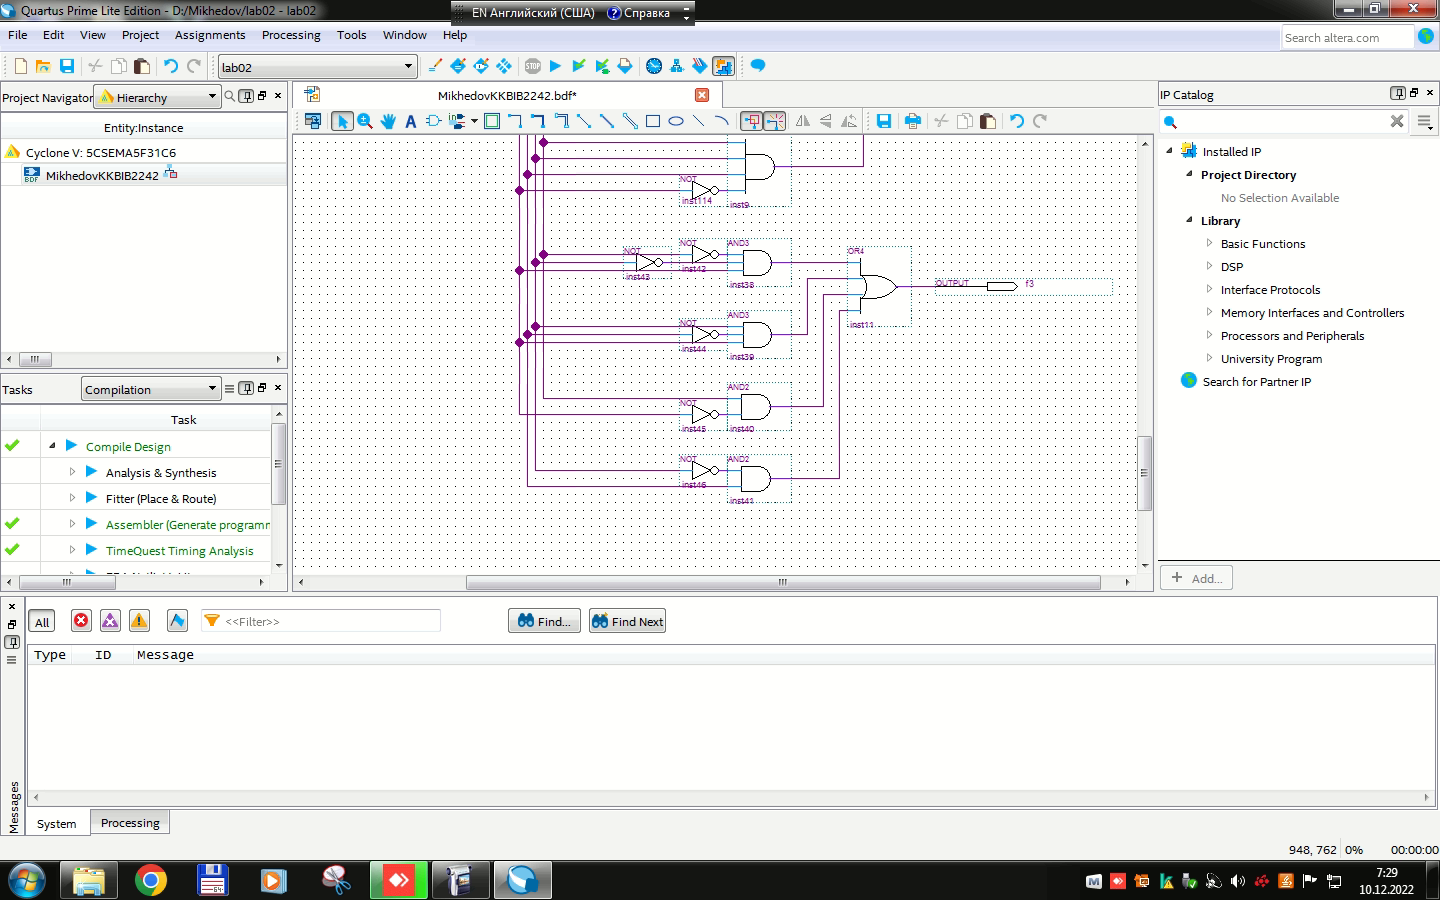
\includegraphics[width=0.95\textwidth]{02_40}
    \caption{схема упрощенного выражения}
  \end{figure}

  И снова запустить функциональную симуляцию:
  \begin{figure}[H]
    \centering
    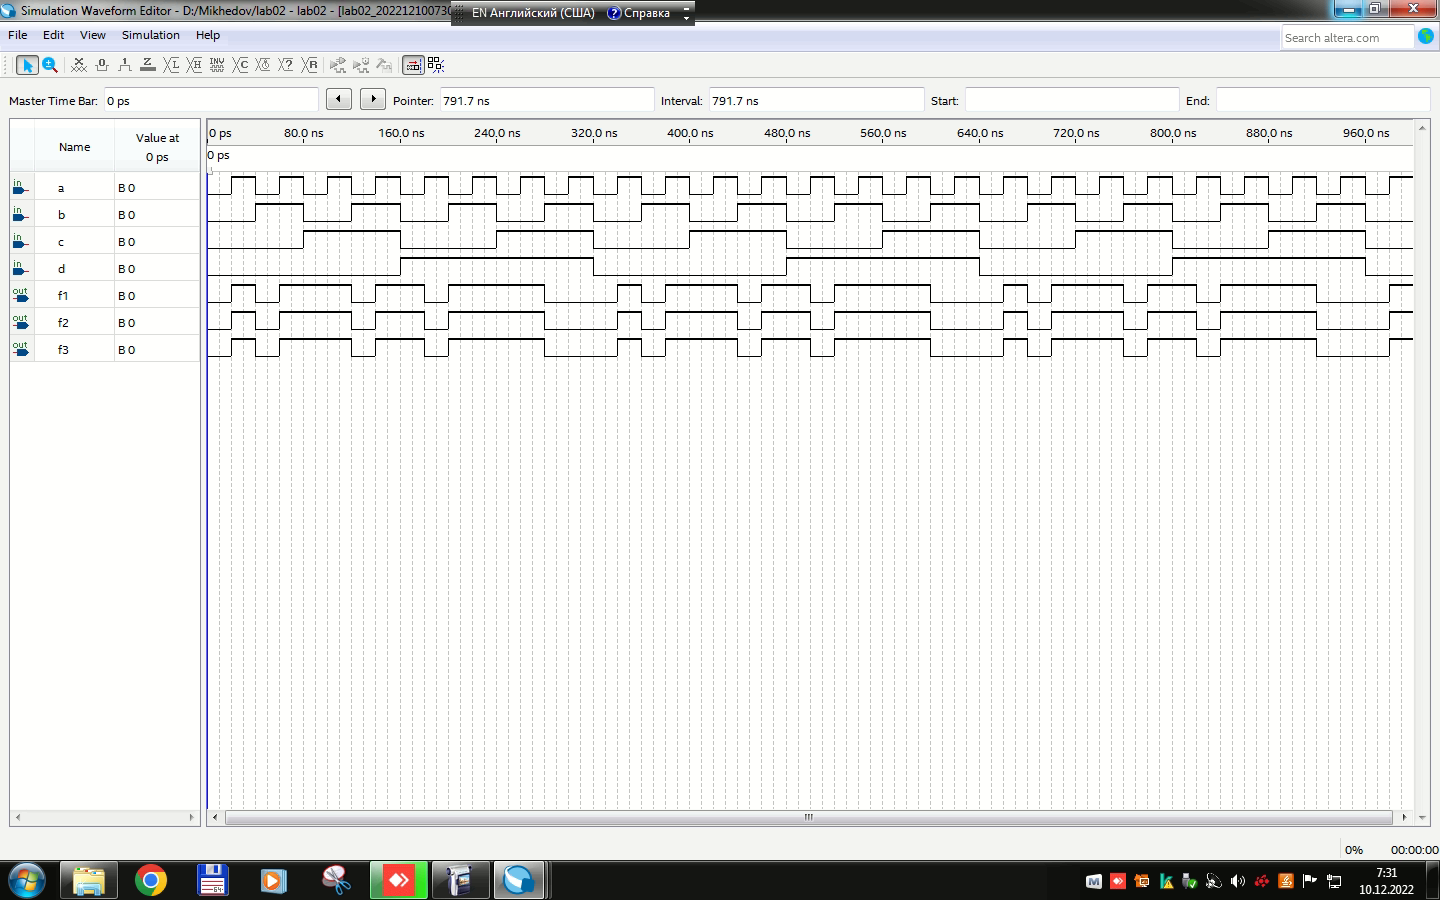
\includegraphics[width=0.75\textwidth]{02_41}
    \caption{результаты функциональной симуляции}
  \end{figure}

  Видно, что значения на фыходах одинаковы и полностью совпадают с таблицей истинности, значит
  все построенно верно.

  \section*{Пункт 5}

  Для оценки задержек необходимо запустить временную симуляцию

  \begin{figure}[H]
    \centering
    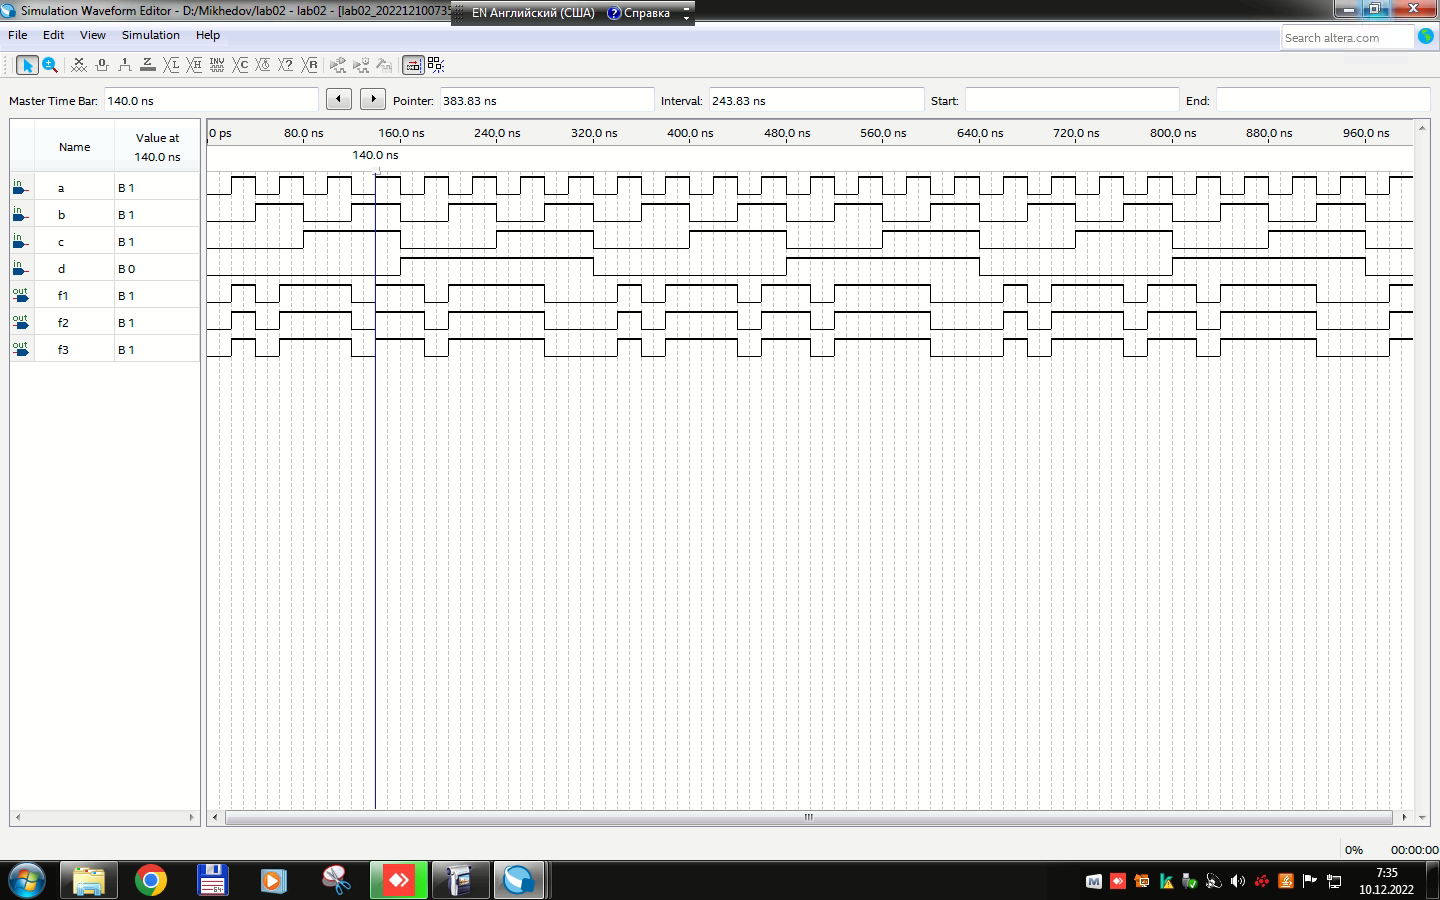
\includegraphics[width=0.75\textwidth]{02_50}
    \caption{результаты временной симуляции}
  \end{figure}

  Видно, что все 3 схемы работают практически мгновенно

  \section*{Пункт 6}

  Для демонстрации работы платы необходимо задать правильные пины. Для выходов использовались
  светодиоды ledr0, ledr1 и ledr2, а в качестве входов - виртуальные кнопки (GPIO порты) с
  номерами от 1 до 4 (включительно)

  \begin{figure}[H]
    \centering
    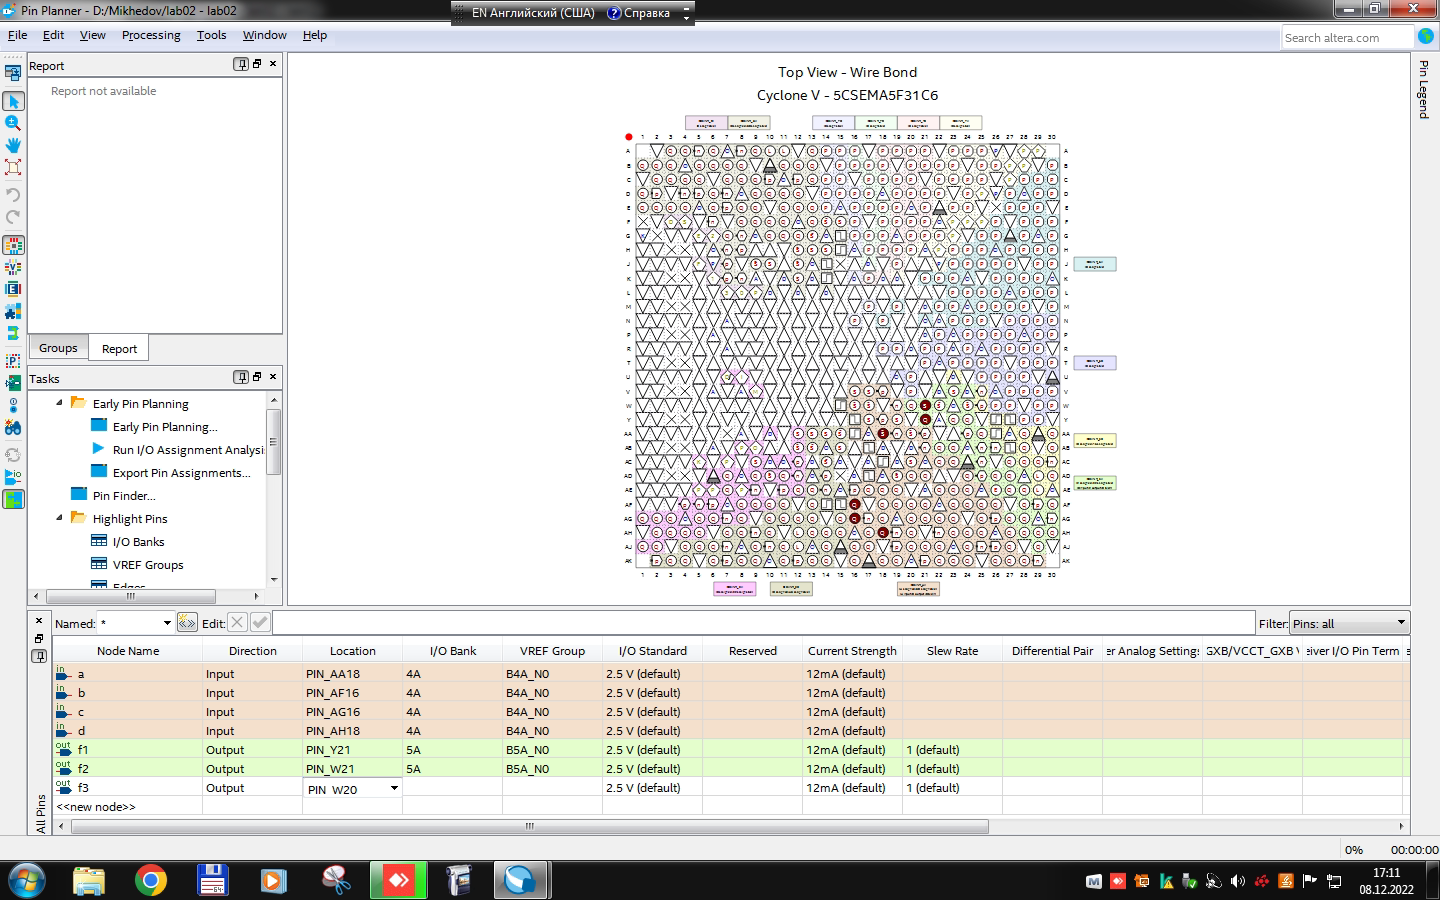
\includegraphics[width=0.75\textwidth]{02_60}
    \caption{назначенные пины}
  \end{figure}

  Далее необходимо скомпилировать проект и прошить плату

  \begin{figure}[H]
    \centering
    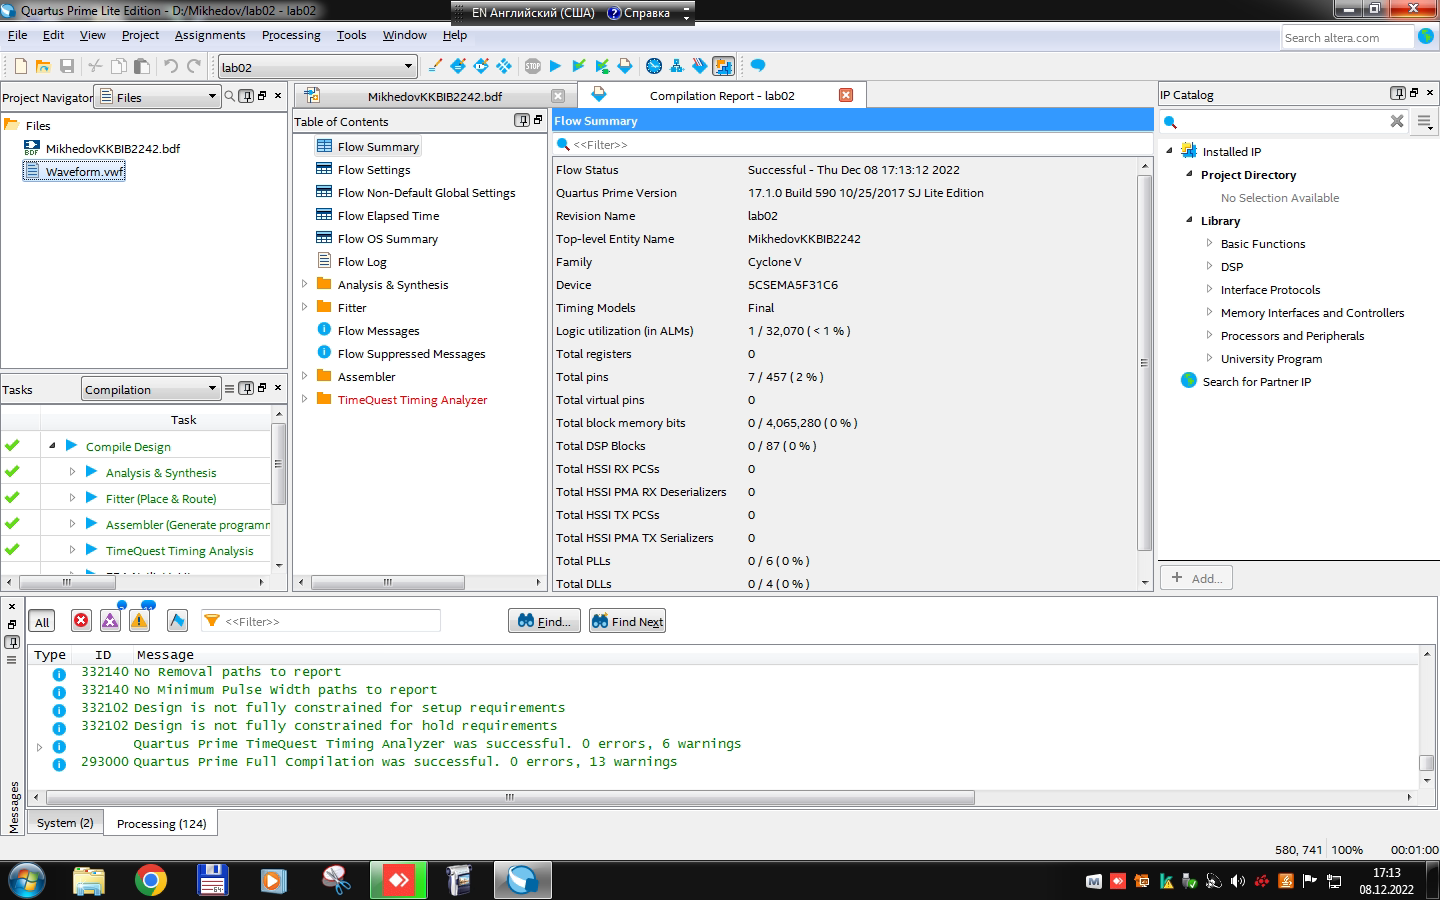
\includegraphics[width=0.8\textwidth]{02_61}
    \caption{компиляция проекта}
  \end{figure}

  \begin{figure}[H]
    \centering
    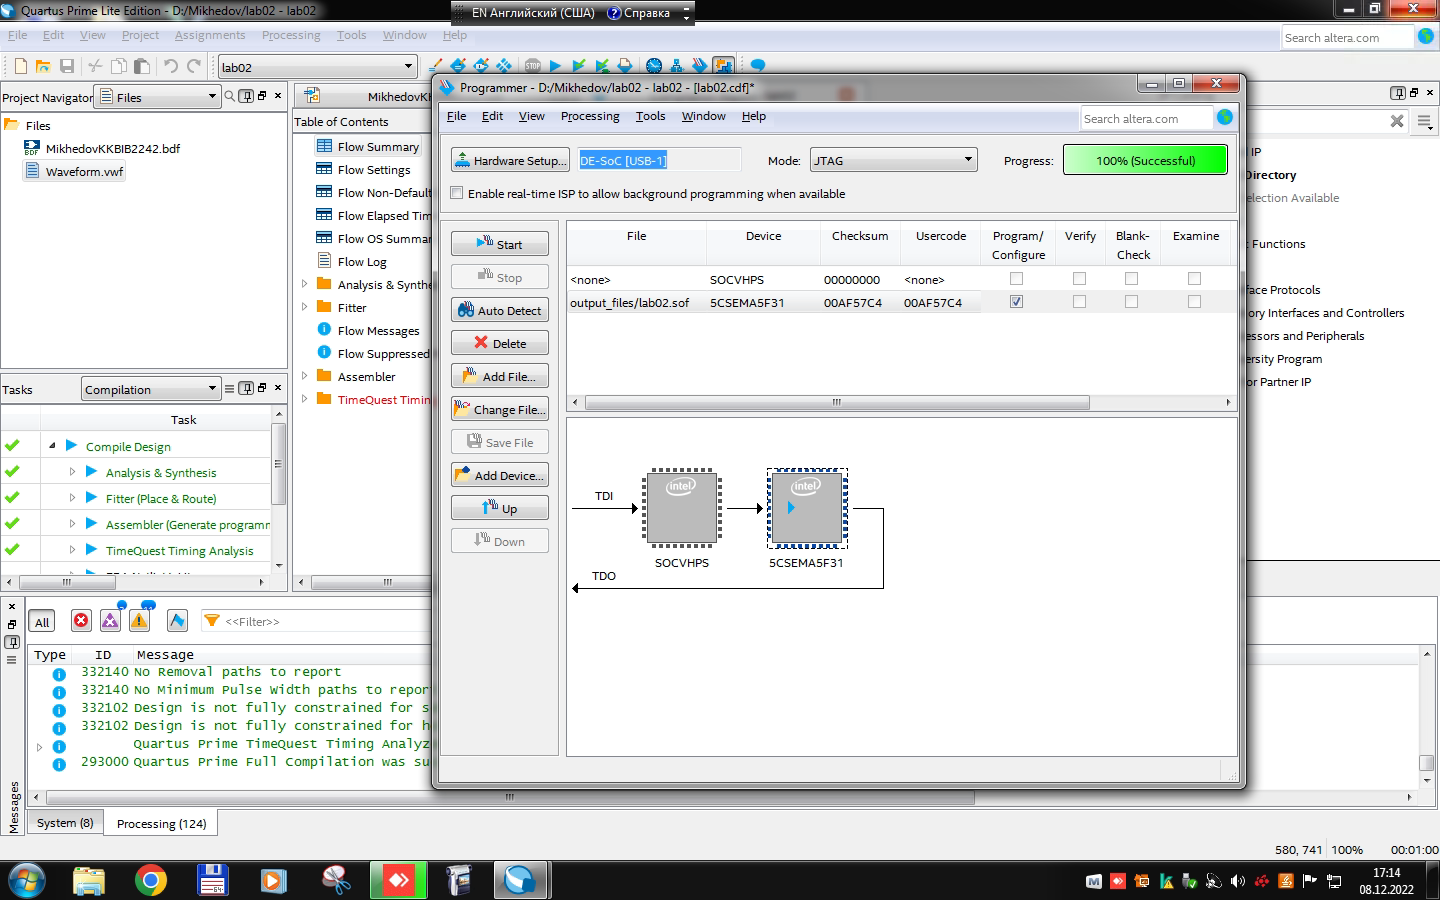
\includegraphics[width=0.8\textwidth]{02_62}
    \caption{прошивка платы}
  \end{figure}

  Теперь подключаемся к плате и проверяем ее работоспособность

  \begin{figure}[H]
    \centering
    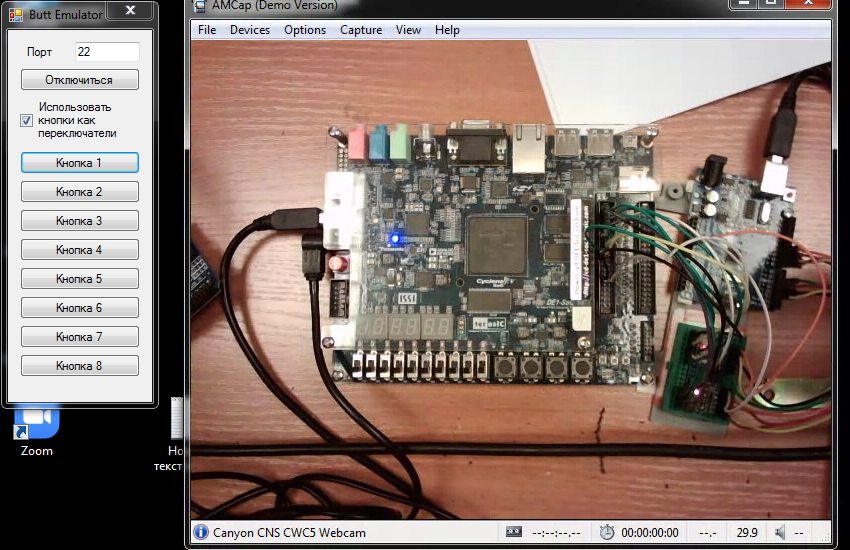
\includegraphics[width=0.335\textwidth, angle=90]{02_70}
    \hfill
    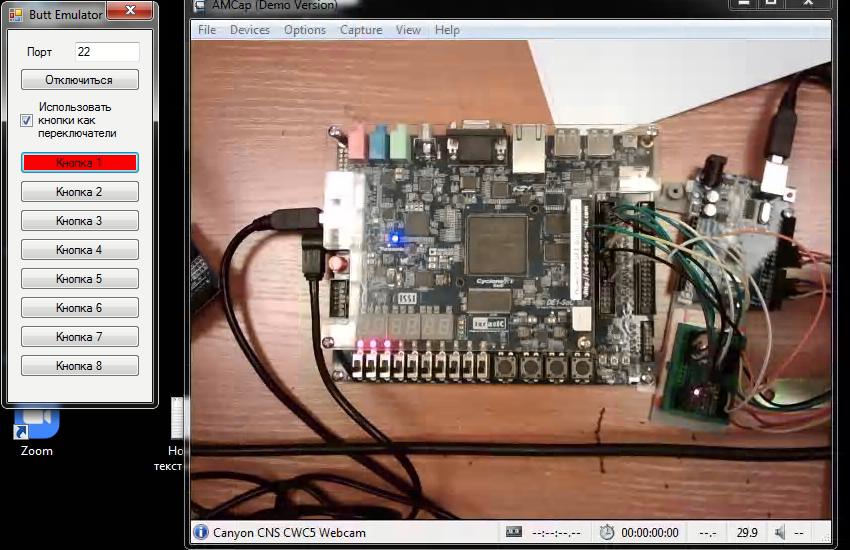
\includegraphics[width=0.335\textwidth, angle=90]{02_71}
    \hfill
    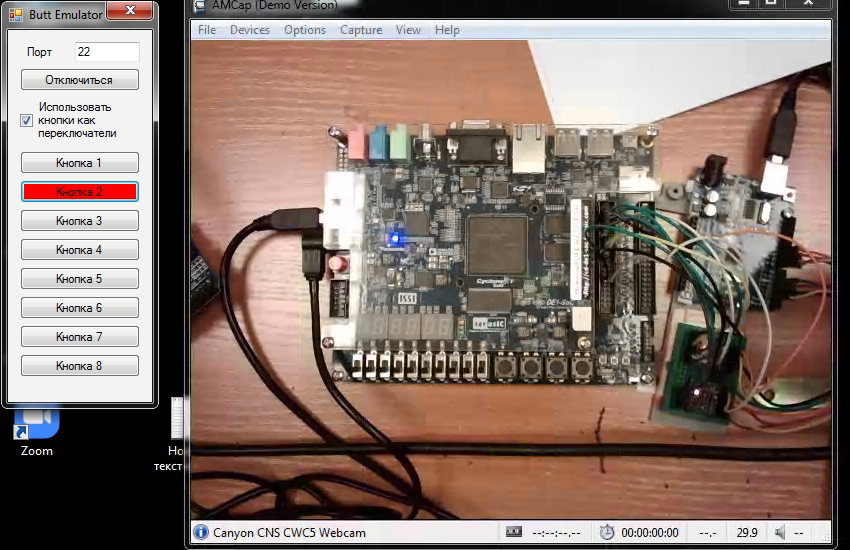
\includegraphics[width=0.335\textwidth, angle=90]{02_72}
    \hfill
    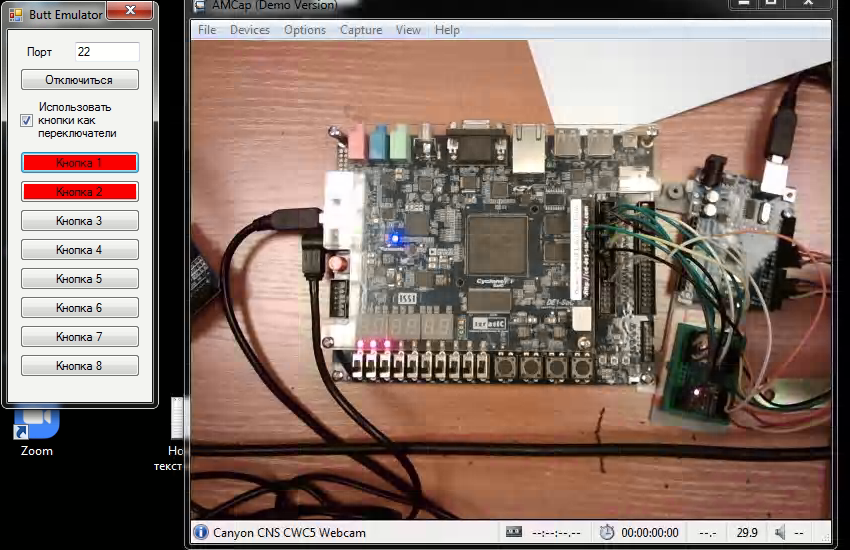
\includegraphics[width=0.335\textwidth, angle=90]{02_73}
    \vspace{0.15cm}

    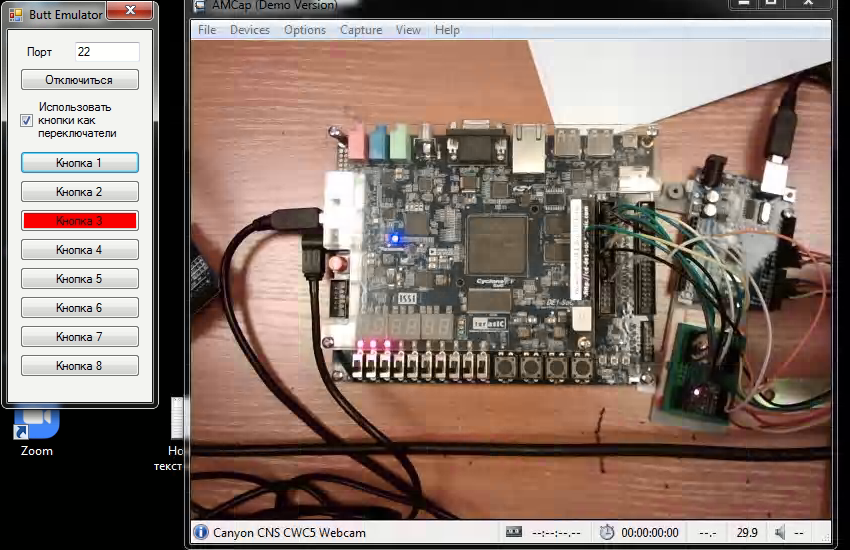
\includegraphics[width=0.335\textwidth, angle=90]{02_75}
    \hfill
    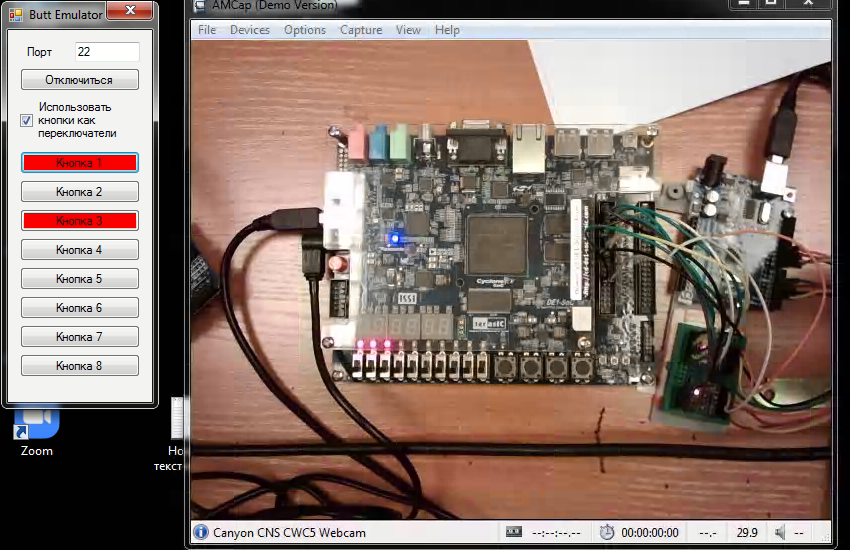
\includegraphics[width=0.335\textwidth, angle=90]{02_76}
    \hfill
    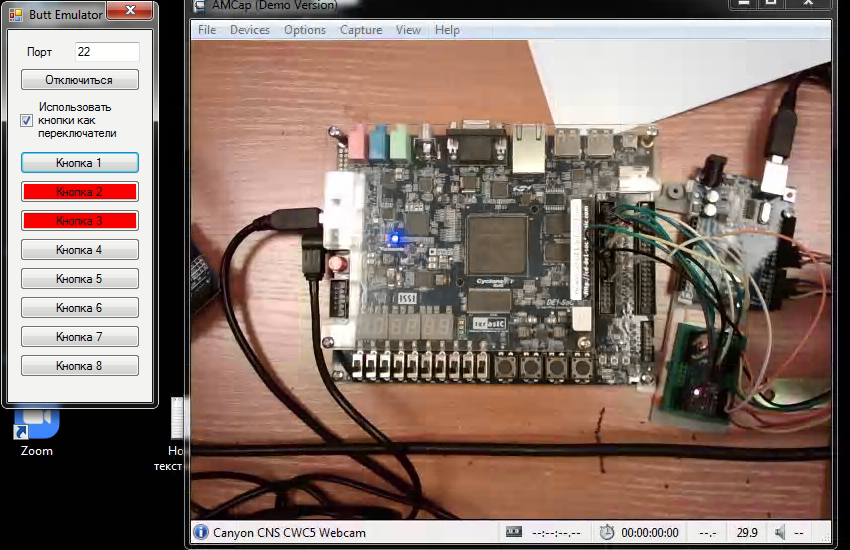
\includegraphics[width=0.335\textwidth, angle=90]{02_77}
    \hfill
    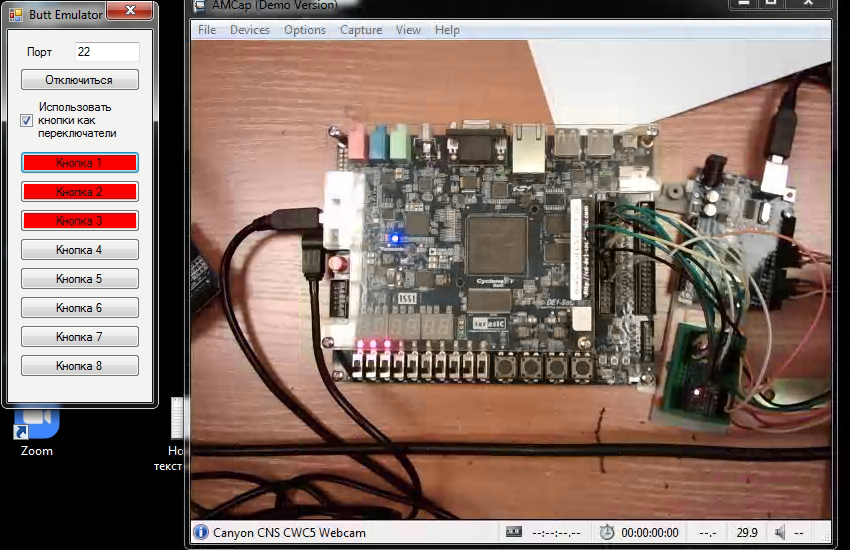
\includegraphics[width=0.335\textwidth, angle=90]{02_78}
    \vspace{0.15cm}

    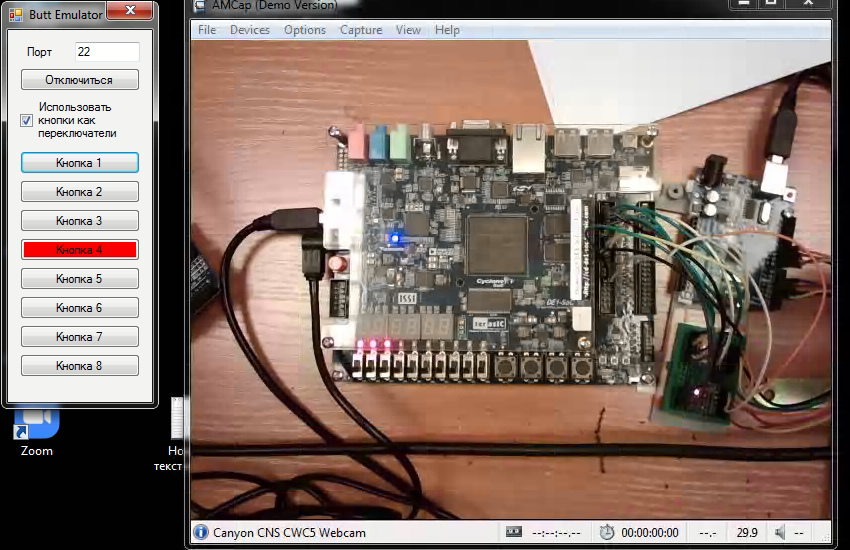
\includegraphics[width=0.335\textwidth, angle=90]{02_79}
    \hfill
    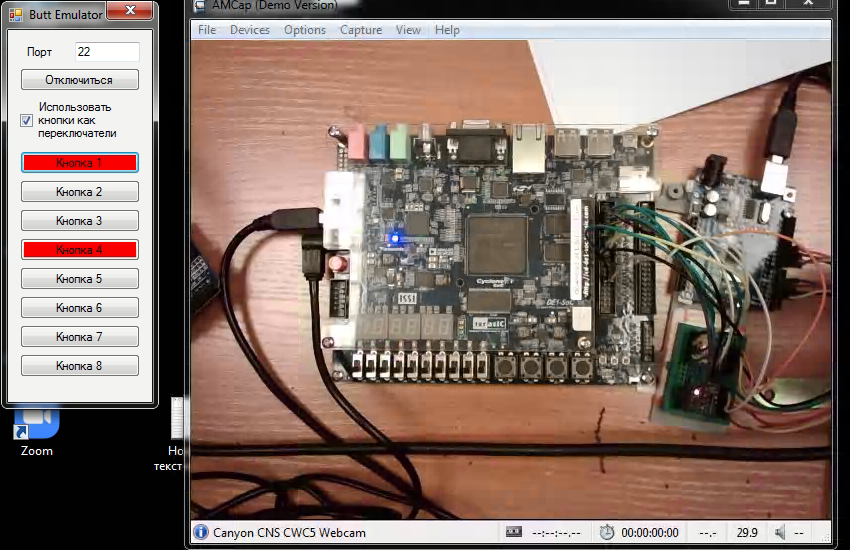
\includegraphics[width=0.335\textwidth, angle=90]{02_80}
    \hfill
    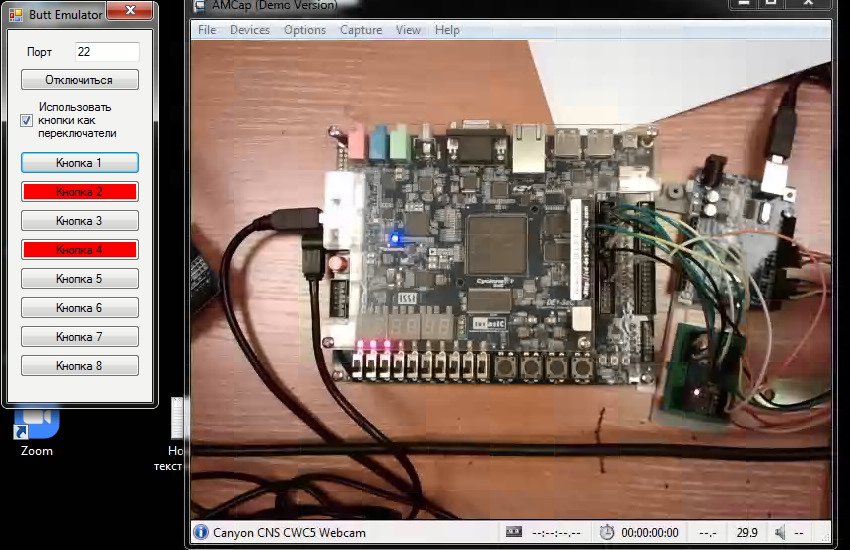
\includegraphics[width=0.335\textwidth, angle=90]{02_81}
    \hfill
    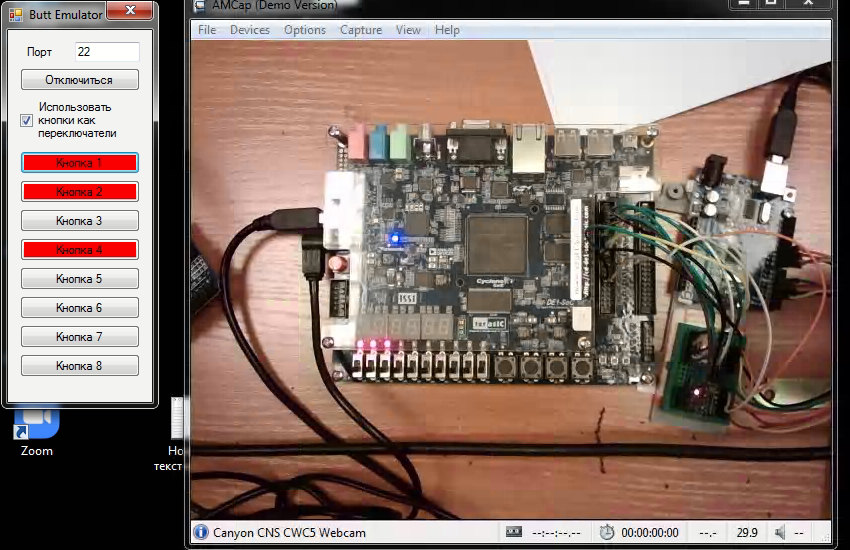
\includegraphics[width=0.335\textwidth, angle=90]{02_82}
    \vspace{0.15cm}

    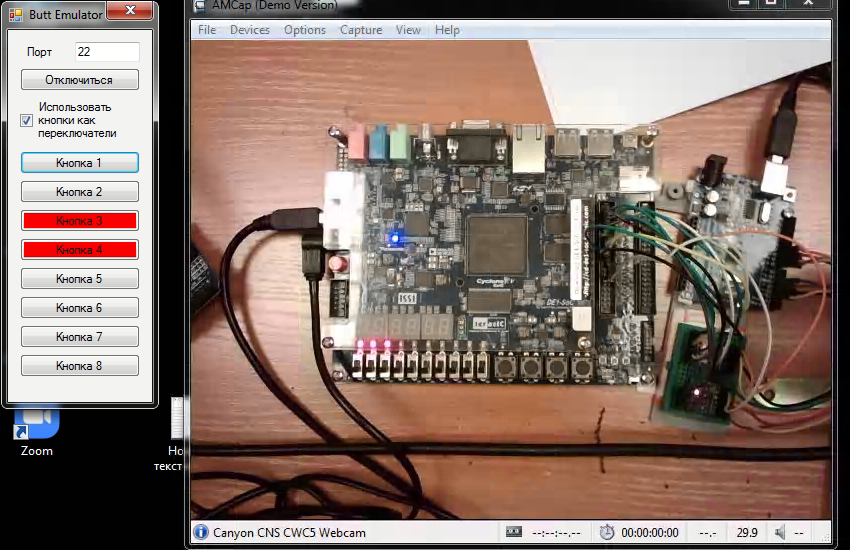
\includegraphics[width=0.335\textwidth, angle=90]{02_83}
    \hfill
    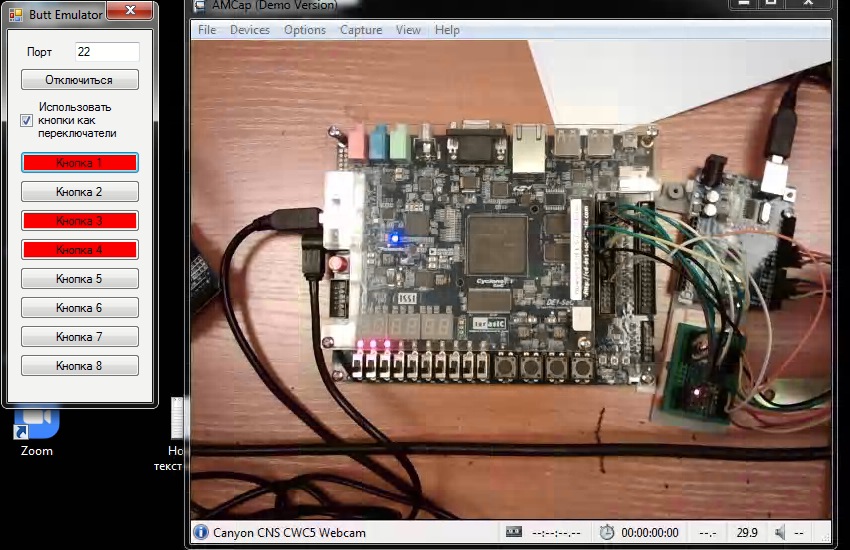
\includegraphics[width=0.335\textwidth, angle=90]{02_84}
    \hfill
    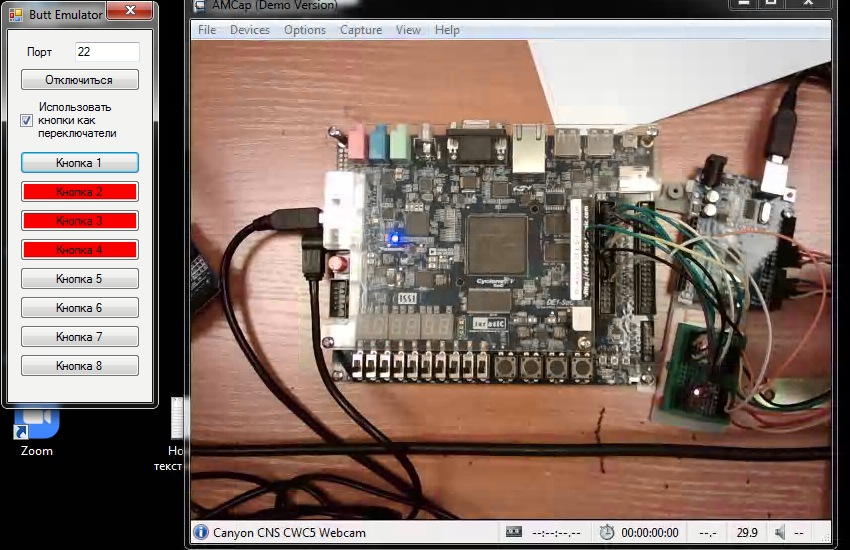
\includegraphics[width=0.335\textwidth, angle=90]{02_85}
    \hfill
    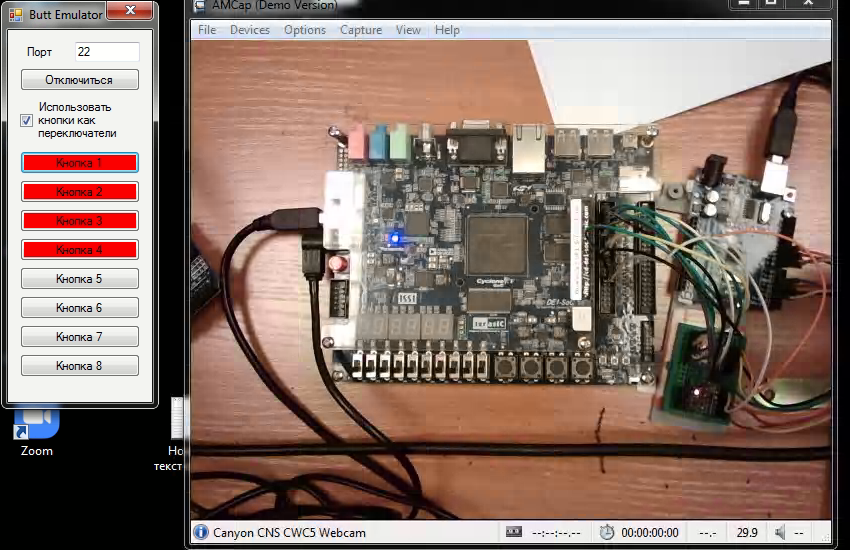
\includegraphics[width=0.335\textwidth, angle=90]{02_86}
    
    \caption{все возможные варианты входных значений}
  \end{figure}

  \section*{Вывод}

  В ходе практической работы мне удалось составить СКНФ и СДНФ по таблице истинности, упростить
  полученные выражения методом Квайна-Мак-Класски, составить эти выражения при помощи логических
  элементов и запустить их на плате.

\end{document}
